%%%%%%%%%%%%%%%%%%%%%%%%%%%%%%  IEEEsample.tex
%%%%%%%%%%%%%%%%%%%%%%%%%%%%%%%%%%%%%%%%%
%%%%%%%%%%%%%%%%%%%%%%%    More information: see the header of IEEEtran.sty
%%%%%%%%%%%%%%%%%%%%%%%
%%%%%%%%%%%%%%%%%%%%%%%%%%%%%%%%%%%%%%%%%%%%%%%%%%%%%%%%%%%%%%%%%%%%%%%%%%%%%%%%
%%%%

\documentclass[10pt,twoside]{IEEEtran}
%\documentclass[conference]{IEEEtran}

%%%\IEEEoverridecommandlockouts

\usepackage[ruled,linesnumbered]{./algorithm2e}
%%for algorithm2e package, label has to be following caption in the same line!!!
\renewcommand{\algorithmcfname}{ALGORITHM}
\SetAlFnt{\small}
\SetAlCapFnt{\small}
\SetAlCapNameFnt{\small}
\SetAlCapHSkip{0pt}
\IncMargin{-\parindent}

%% \RequirePackage{times}
%% \RequirePackage{algorithmic}
%% \PassOptionsToPackage{boxed}{algorithm}
%% \RequirePackage{algorithm}
%% \RequirePackage{multicol}
%\renewcommand{\algorithmicrequire}{\textbf{Inputs:}}
%\renewcommand{\algorithmicensure}{\textbf{Outputs:}}
%\DeclareMathAlphabet{\mathtsl}{OT1}{ptm}{m}{sl}

%\def\BibTeX{{\rm B\kern-.05em{\sc i\kern-.025em b}\kern-.08em1
%    T\kern-.1667em\lower.7ex\hbox{E}\kern-.125emX}}

%\newtheorem{theorem}{Theorem}
%\newtheorem{lemma}{Lemma}
%\newtheorem{example}{Example}
%\newtheorem{corollary}{Corollary}

\RequirePackage{amssymb, mathptm}
\usepackage{amsbsy}
\usepackage{amsthm}
\usepackage{graphicx}
\usepackage{helvet}
\usepackage{enumerate}
\usepackage{amsmath}
\usepackage{amsfonts}
\usepackage{graphicx}
\usepackage{multirow}
\usepackage{subfig}
\usepackage{cases}
\usepackage{comment}



%%indent in algorithm


%\setcounter{page}{1}


% New command for the table notes.
\def\tabnote#1{{\small{#1}}}

% New command for the line spacing.
\newcommand{\ls}[1]
    {\dimen0=\fontdimen6\the\font
     \lineskip=#1\dimen0
     \advance\lineskip.5\fontdimen5\the\font
     \advance\lineskip-\dimen0
     \lineskiplimit=.9\lineskip
     \baselineskip=\lineskip
     \advance\baselineskip\dimen0
     \normallineskip\lineskip
     \normallineskiplimit\lineskiplimit
     \normalbaselineskip\baselineskip
     \ignorespaces
    }
%\renewcommand{\algorithmicrequire}{\textbf{Input:}}
%\renewcommand{\algorithmicensure}{\textbf{Output:}}

\newcommand{\beq}{\begin{equation}}
\newcommand{\eeq}{\end{equation}}
\newcommand{\beqarr}{\begin{eqnarray}}
\newcommand{\eeqarr}{\end{eqnarray}}
%\newcommand{\ov}{\overline}
\newcommand{\ov}{\bar}
\newcommand{\xor}{\bigoplus}
\newcommand{\Fm}{{\mathbb{F}}}



%the following is for space before and after align or other equation environment.

%%
\newtheorem{Algorithm}{Algorithm}[section]
\newtheorem{Definition}{Definition}[section]
\newtheorem{Example}{Example}[section]
\newtheorem{Proposition}{Proposition}[section]
\newtheorem{Lemma}{Lemma}[section]
\newtheorem{Theorem}{Theorem}[section]
\newtheorem{Corollary}{Corollary}[section]
\newtheorem{Conjecture}{Conjecture}[section]
\newtheorem{Problem}{Problem}[section]
\newtheorem{Notation}{Notation}[section]
\newtheorem{Setup}{Problem Setup}[section]

%%%

%%set spacing between table columns
\setlength{\tabcolsep}{3pt}

\begin{document}

%\thispagestyle{empty}
%\pagestyle{empty}

%\ls{1.5}

\title{\large{\textsc{Word-level Finite State Machine Traversal using Gr\"obner Basis}}}
%\author{Tim Pruss\\
%A Master's Thesis Proposal\\
%Electrical \& Computer Engineering, University of Utah\\
%Spring Semester 2013
%}

\author{

\IEEEauthorblockN{Xiaojun Sun\IEEEauthorrefmark{1}, Priyank
  Kalla\IEEEauthorrefmark{1}, Florian Enescu\IEEEauthorrefmark{2}\\}
%\thanks{This work is sponsored in part by a grant from NSF \#CCF-546859.}
\IEEEauthorblockA{\IEEEauthorrefmark{1}Electrical \& Computer
  Engineering, University of Utah\\
\IEEEauthorrefmark{2}Mathematics \& Statistics, Georgia State
University \vspace{-0.25in}
 \{xiaojuns, kalla\}@ece.utah.edu, fenescu@gsu.edu
}
%% \and
%% \IEEEauthorblockN{Florian Enescu\\} 
%% %\thanks{\normalsize  978-3-9810801-8-6/DATE12/$\copyright 2012$ EDAA}
%% \IEEEauthorblockA{Mathematics \& Statistics, Georgia State University
%% % fenescu@mathstat.gsu.edu
%% } 
}
 
\maketitle

%\markboth{MS Proposal by Tim Pruss}{}
\newcommand{\Fq}{{\mathbb{F}}_{q}}
\newcommand{\Fkk}{{\mathbb{F}}_{2^k}}
\newcommand{\Fkkx}[1][x]{\ensuremath{\mathbb{F}}_{2^k}[#1]\xspace}
\newcommand{\Grobner}{Gr\"{o}bner\xspace}
\newcommand{\B}{{\mathbb{B}}}
\newcommand{\Z}{{\mathbb{Z}}}
\newcommand{\F}{{\mathcal{F}}}
\newcommand{\G}{{\mathcal{G}}}
%%%

\newcommand{\debug}[1]{\textcolor{gray}{[ #1 ]}}


%\thispagestyle{empty}
%\pagestyle{empty}

%%%%%%%%%%%%%%%%%%%% Include your files here %%%%%%%%%%%%%%%%%%%%%
%\input{myformulae.tex}


\section{Preliminaries}

\subsection{FSM model for sequential circuits}
A finite state machine (FSM) is a mathematical model of computation for designing and analyzing sequential logic 
circuits. If a FSM's primary outputs depend on primary inputs and present state inputs, it is named as a \textit{Mealy machine};
the formal definition is as follows:
\begin{Definition}
A Mealy machine is an $n$-tuple $\mathcal M = (\Sigma,O,S,S^0,\Delta,\Lambda)$ where
\begin{itemize}
\item $\Sigma$ is the input label, $O$ is the output label;
\item $S$ is the set of states, $S^0\subseteq S$ is the set of initial states;
\item $\Delta:\ S\times\Sigma\to S$ is the next state transition function;
\item $\Lambda:\ S\times\Sigma\to O$ is the output function.
\end{itemize}
\end{Definition}
The other kind of FSM is \textit{Moore machine}, its difference from Mealy machine is that
its primary outputs only depend on the present states, i.e. the output function is defined as
$$\Lambda:\ S \to O$$
Typical sequential circuits can be depicted as Fig.\ref{fig:seqmodel}(a). Primary inputs
$x_1,\dots,x_m \in \Sigma$, and primary outputs $z_1,\dots,z_n\in O$. Signals $s_1,\dots,s_k$ 
are present state (PS) variables, $t_1,\dots,t_k$ are next state (NS) variables.
We can define 2 $k$-bit words denoting the PS/NS variables as there are $k$ flip-flops
in the datapath: $S = (s_1,\dots,s_k), ~T=(t_1,\dots,t_k)$. Transition function
at bit level are defined as $\Delta_i: t_i = \Delta_i(s_1,\dots,s_k,x_1,\dots,x_m)$.
\begin{figure}[hbt]
\centering{
%\begin{minipage}{12cm}
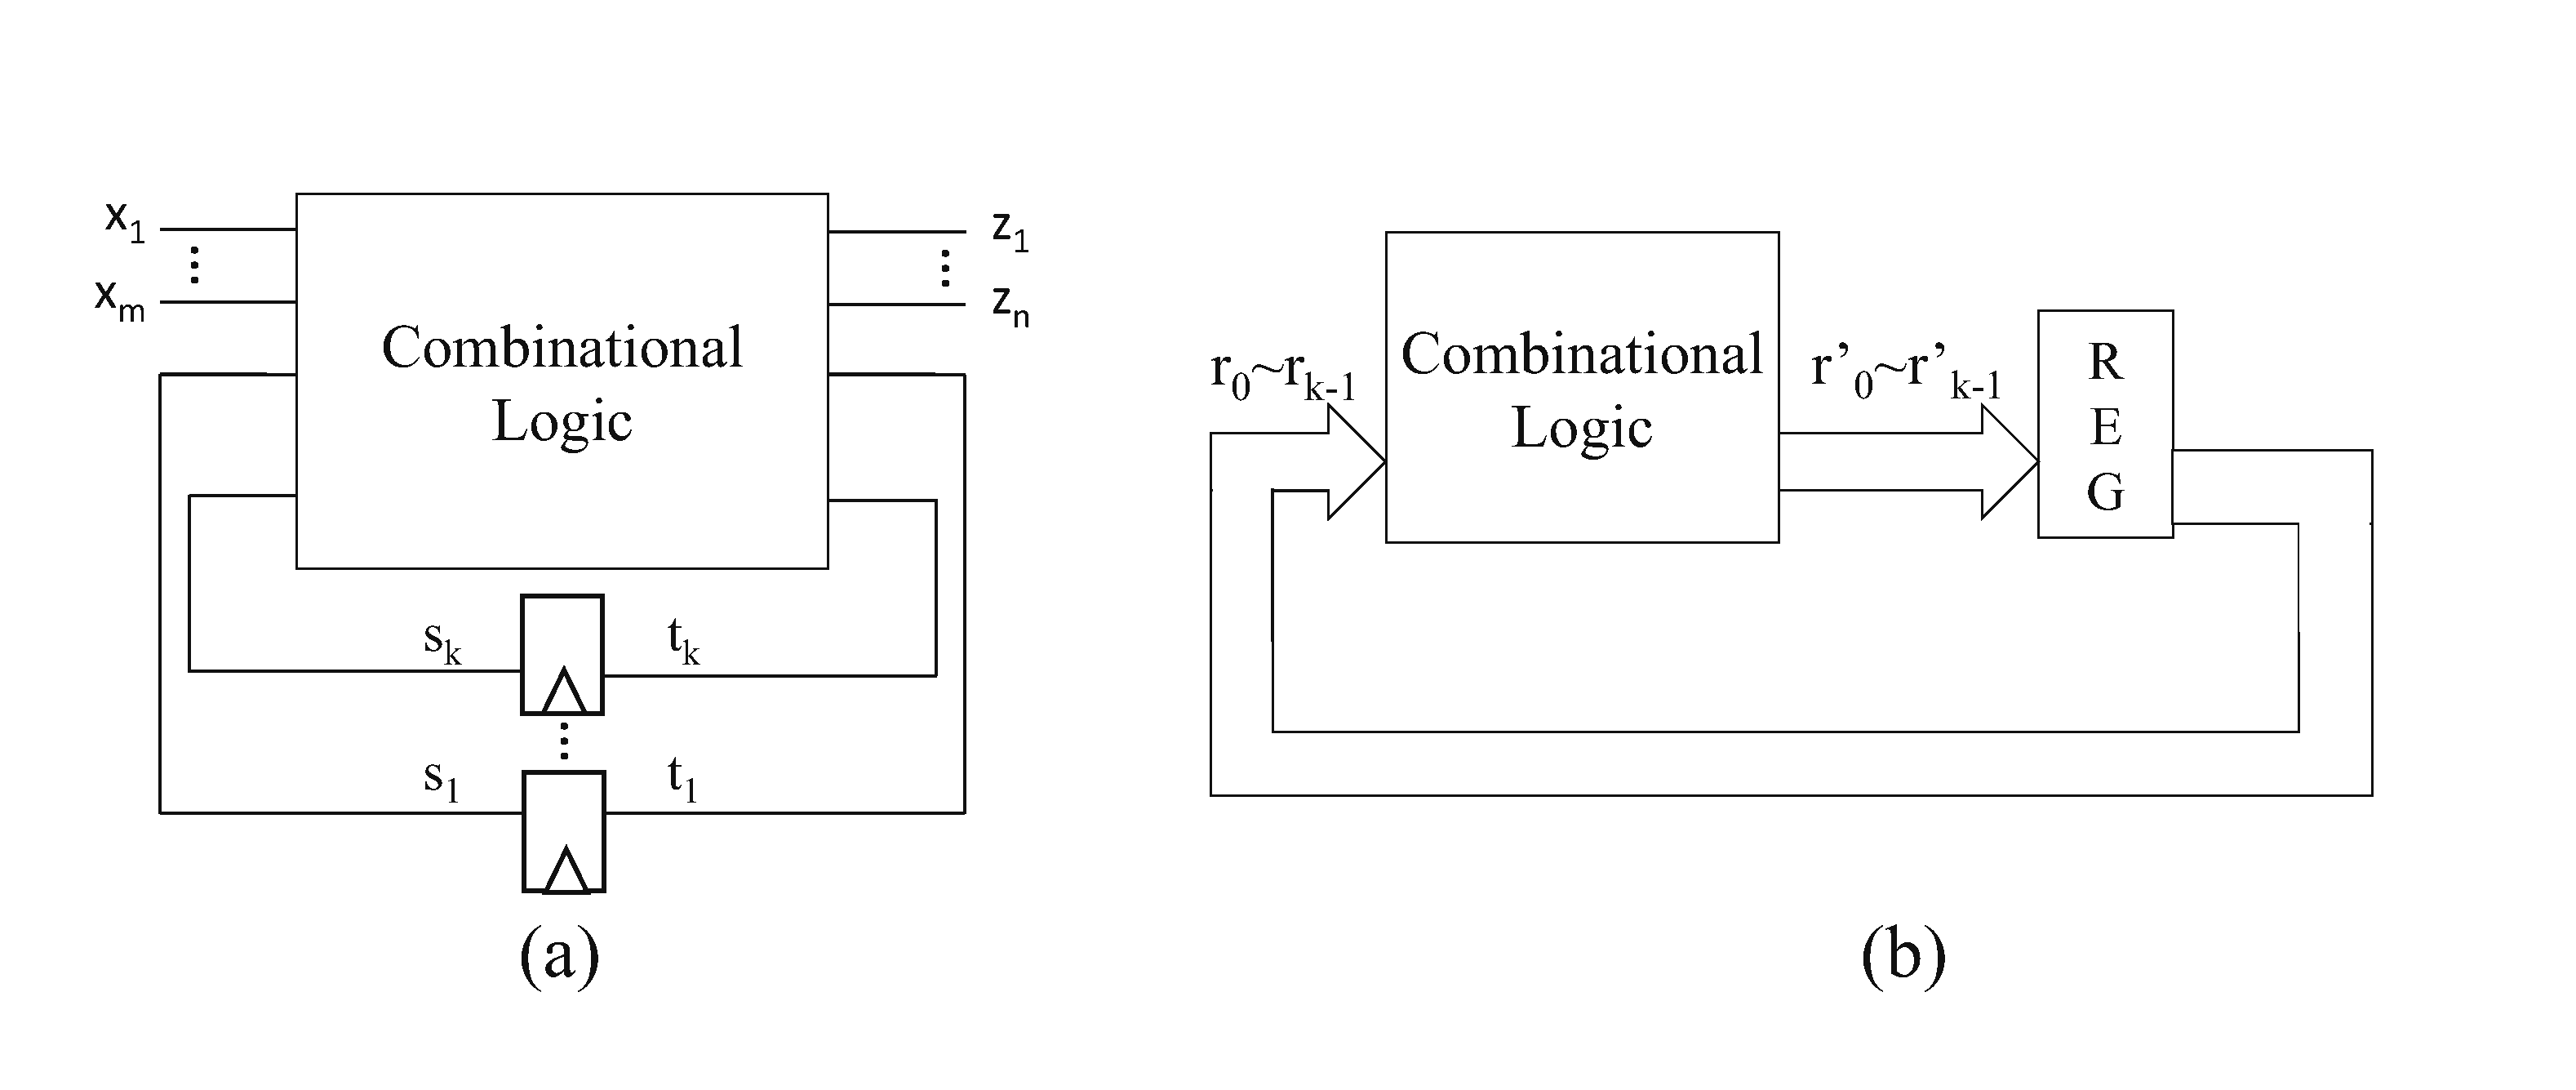
\includegraphics[width=3.5in]{./seqmodel.eps}
% \vspace{-0.2in}
\caption{FSM models of sequential circuits}
%\end{minipage}
\label{fig:seqmodel}}
\end{figure}
In some cases, arithmetic computations are implemented as Moore machines where input operands
are loaded into register files $R$ and the FSM is executed for $k$ clock cycles.
We can simplify them to the model in Fig.\ref{fig:seqmodel}(b).

\subsection{Commutative algebra and algebraic geometry preliminaries}
A {\bf field} $\mathbb{F}$ is a set of elements, including 0 and 1 (unity),
allowing for associative and commutative addition and multiplication;
and every non-zero element has a multiplicative inverse.  A {\bf
  finite field} or {\bf Galois filed} is a field with a finite number
($q$) of elements, and is denoted by $\Fq$, where $q=p^k$ is a power of
a prime integer $p$. In our work, $q = 2^k$ for
a given $k$, where $k$ represents the datapath (bit-vector)
word-lengths, or the number of memory elements (state registers) in
finite state machines. 

Let the field $\mathbb{F}_2 = \{0, 1\} ~(\equiv \B)$, and let
$\mathbb{F}_2[X]$ denote the set (ring) of all univariate polynomials
in variable $X$ with coefficients from $\mathbb{F}_2$. Then, the
Galois field $\Fkk$ is constructed as $\Fkk = \mathbb{F}_2[X] \pmod{
  P(X)}$, where $P(X)$ is an irreducible polynomial over
$\mathbb{F}_2$. Let $\alpha$ be a root of the irreducible polynomial
$P(X)$, i.e. $P(\alpha) = 0$. Any element $A \in \Fkk$ can be
represented as $A = \sum_{i=0}^{k-1} a_i \alpha^i$, where $a_i \in
\mathbb{F}_2$. The field $\Fkk$ is therefore, a $k$-dimensional {\it
  extension} of the base field $\mathbb{F}_2$: so,  $\mathbf{\Fkk \supset
\mathbb{F}_2}$. Consequently, all operations of addition and
multiplication in $\Fkk$ are performed modulo the irreducible
polynomial $P(\alpha)$ and coefficients are reduced modulo 2.  

Boolean variables in field $\mathbb B$ can be easily mapped to
elements in $\mathbb F_2$. Since $\mathbb F_2 \subset \Fkk$, these 
%Namely $k$-bit Boolean bit-vector defined
%over Boolean ring $\mathbb B^k$ can also be mapped uniquely  to $\Fkk
%= \mathbb F_2[x_1,\dots,x_k]$. 
Boolean operators are interpreted as functions over $\Fkk$ (where $+$
and $\cdot$ are addition and multiplication performed modulo 2): 
\begin{align*}
&a\land b \to a\cdot b\\
&a\oplus b \to a+b\\
&\neg a \to 1+a\\
&a \bar{\oplus} b \to 1+a+b\\
&a \lor b \to a+b+a\cdot b
\end{align*}

Using these mappings we can write Boolean functions in form of
polynomials over $\mathbb F_2\subset \Fkk$. 
These concepts provide a mechanism to represent and
manipulate both bit-level ($\mathbb{F}_2$) and $k$-bit word-level
constraints {\bf in one unified mathematical domain $\Fkk$ --- a
  concept we   exploit for abstraction. }
  Consider Ex.\ref{ex:motiv},
polynomials for transition functions (bit-level outputs) $f_1,f_2$
are over $\mathbb F_2$, i.e. $f_1,f_2\subseteq \mathbb F_2 \subset \Fkk$,
and polynomials containing word-level variables $f_3,f_4,f_5 \subseteq \Fkk$.
All polynomials belong to unified domain $f_1,f_2,\dots,f_5 \subseteq \Fkk$.

It is well-known that every Boolean mapping between $k$ dimensional
Boolean spaces $f: \B^k \rightarrow \B^k$ can be construed as a
function over Galois fields $f: \Fkk \rightarrow \Fkk$. Moreover,
every function $f: \Fkk \rightarrow \Fkk$ is a polynomial function: 
i.e. $f$ can be represented by way of a unique, minimal, canonical
polynomial $\F(X)$, and the work of \cite{timDAC} shows how to
efficiently derive such polynomial representations from circuits ---
another concept that makes our approach feasible. 


We represent Boolean circuits by way of polynomials over
$\Fkk$. If we take indeterminates $x_1,x_2,\dots,x_n$, an arbitrary
combination of their finite product  
$x_1^{d_1}\cdot x_2^{d_2}\cdots x_n^{d_n}, d_i\geq 0$ 
is a {\bf monomial}. A {\bf polynomial} $f = c_1 X_1 + c_2 X_2 + \dots
+ c_t X_t$ is a finite sum of terms, where $c_1, \dots, c_t$ are
coefficients and $X_1, \dots, X_t$ are monomials. The set of {\it all}
such polynomials with coefficients from $\Fkk$ forms a {\bf
  multivariate polynomial ring} denoted $\Fkk[x_1,\dots,x_n]$. 
A monomial ordering $X_1 > X_2 \dots > X_t$ is imposed on the
polynomials to process them systematically. Then, $LT(f) = c_1 X_1,
LM(f) = X_1$ denote the leading term and the leading monomial of $f$,
respectively. 


Multivariate polynomial division will play a key role in our
algorithmic techniques. Division is implemented as {\it cancellation
  of terms.} Given polynomials $f, g$, if $cX$ is a term in
$f$ that is divisible by $LT(g)$, then $f \xrightarrow{g} r$ denotes a
one-step reduction (division) of $f$ by $g$, resulting in remainder $r
= f - {{cX} \over {LT(g)}} \cdot g$. This has the effect of cancelling
the term $cX$ from $f$. 
\begin{Example}
\label{ex:multidiv}
If $f = e + cd$ and $g = c + ab$,
then the term $cd$ in $f$ can be canceled by $LT(g) = c$: $r = f - {cd
  \over c} g = e + abd$. 
\end{Example}
  Similarly, $f$ reduces to $r$ modulo the set
of polynomials $F = \{f_1, \dots, f_s\}$, denoted $f \stackrel{F}
{\textstyle   \longrightarrow}_+ r$, such that no term in $r$ is
divisible (cancellable) by the $LT(f_i)$ of any polynomial in $ f_i
\in F$.    


In verification, we have to analyze the {\it solutions to a
set of polynomials.} The set of all solutions to a system of
polynomial equations $f_1 = \dots = f_s = 0$ is defined as the affine variety:
\begin{Definition}
Given a set of polynomials $f_1,\dots,f_s$ over ring $\mathbb F_q[x_1,\dots,x_n]$, their 
{\bf affine variety} 
$$V(f_1,\dots,f_s) = \{(a_1,\dots,a_n)\in  (\mathbb F_q)^n |
f_1(a_1,\dots,a_n) = \cdots = f_s(a_1,\dots,a_n) = 0\}$$ 
\end{Definition}

Generally we can find many sets of polynomials with the same variety, which are linear combinations
of given set of polynomials. This set is defined as follows:
\begin{Definition}
{\bf Ideal of Polynomials:} Let $f_1,f_2,\dots,f_s\in \mathbb F[x_1,\dots,x_n]$.
Define an ideal
$$J = \langle f_1,f_2,\dots,f_s\rangle = \{f_1\cdot h_1 + f_2\cdot h_2 +\cdots + f_s\cdot h_s : h_1,\dots,h_s\in \mathbb F[x_1,\dots,x_n]\}$$
We call $J = \langle f_1,f_2,\dots,f_s\rangle$ an ideal generated by $f_1,\dots,f_s$ and these polynomials 
the {\bf generators} of ideal $J$.
\end{Definition}
% On the other hand, if given another polynomial $f$, we need to judge whether it belongs to $J$.
A practical problem is: given an ideal $J = \langle f_1,f_2,\dots,f_s\rangle$ and a polynomial $f$,
we need to check if the variety of $J$ can make the evaluation of $f$ equal to 0, i.e. $f$ vanishes on $V(J)$.
This problem is usually described as ideal membership checking problem.
\begin{Definition}
{\bf Ideal membership:} Let $f_1,f_2,\dots,f_s\in \mathbb F[x_1,\dots,x_n]$, and $J = \langle f_1,f_2,\dots,f_s\rangle$
be an ideal over ring $\mathbb F[x_1,\dots,x_n]$. If 
$$f = f_1h_1 + f_2h_2 + \cdots + f_sh_s$$
then $f\in J$.
\end{Definition}

An ideal may have many generating sets. For example, we may have different set of polynomial generators denoting
the same ideal, where they have the same variety: $\langle f_1,\dots,f_s\rangle = \langle h_1,\dots,h_r\rangle
= \langle g_1,\dots,g_t\rangle$ such that $V(f_1,\dots,f_s) = V(h_1,\dots,h_r) = V(g_1,\dots,g_t)$.
Therefore a canonical representation of an ideal is needed, which leads to the concept of Gr\"obner bases.

\begin{Definition}
The set $G = \{g_1, \dots,
g_t\}$ is called a \textbf{\Grobner basis} of $J$ if and only if the
leading term of all polynomials in $J$ is divisible be the leading
term of some polynomial $g_i$ in $G$: i.e. $\forall f \in J, \exists
g_i \in G \ s.t. \ LT(g_i) ~|~ LT(f)$. 
\end{Definition}
% The famous Buchberger's
% algorithm, given in textbook \cite{ideals:book}, is used to compute a
% \Grobner basis (GB). Operating on  input $F = \{f_1, \dots, f_s\}$,
% and subject to the imposed term order $>$, it derives $G = GB(J) = \{
% g_1, \dots, g_t \}$. Buchberger's algorithm repeatedly computes
% $S$-polynomials. For pairs $(f_i, f_j) \in F$, $Spoly(f_i, f_j) =
% \frac{L}{lt(f_i)}\cdot f_i - \frac{L}{lt(f_j)}\cdot f_j$, where $L =
% LCM(LM(f_i), LM(f_j))$. Reducing $Spoly(f_i, f_j) \xrightarrow{F}_+ r$
% cancels the leading terms of $f_i, f_j$ and gives a polynomial $r$
% with a new leading term. This remainder $r$ is added to the current
% basis and $Spoly(f_i, f_j)$ computations are repeated for all pairs of
% polynomials until all $S$-polynomials reduce to 0.  

An advantage of representing an ideal with GB is that it can serve as a decision procedure for ideal membership
test when dividing a polynomial $f$ by a GB, i.e.
$$G = GB(J) \Longleftrightarrow \forall f\in J, f\xrightarrow{g_1,g_2,\dots,g_t}_{+} 0$$
Gr\"obner basis can be reduced by eliminating redundant elements. \textbf{A reduced GB is a canonical representation of 
the ideal under a given monomial ordering}. Given an ideal $J = \langle f_1,\dots,f_s\rangle, ~G = 
\{g_1,\dots,g_t\}$ is the GB of $J$, it can be computed by Buchberger's algorithm (refer to textbook \cite{ideal:book}).

Another advantage of using GB representation is that GB computation can work as a {\it quantification procedure}.
In the following part we will introduce the concept of \textit{vanishing polynomials}, \textit{elimination ideal}, etc.
as the bases of this theory.

{\it Fermat's little theorem over $\Fq$:} For any $ \alpha \in \mathbb
F_{q}, \alpha^q = \alpha$. Therefore, the polynomial $x^q - x$
vanishes ($=0$) over $\Fq$, and is called a vanishing polynomial. We
denote by $J_0 = \langle x_1^q - x_1, \dots, x_d^q - x_d \rangle$ the
ideal of all vanishing polynomials in $\Fq[x_1, \dots, x_d]$. When $q
= 2^k, x^q - x = x^q + x$ as $-1 = +1$ over $\Fkk$.

Gr\"obner bases can be used to {\it eliminate} (i.e. quantify) variables from an
ideal. Given ideal $J = \langle f_1,\dots,f_s\rangle \subset \mathbb
F_{q}[x_1,\dots,x_d]$, the $l^{th}$ elimination ideal $J_l$ is the
ideal of $\Fq[x_{l+1}, \dots, x_d]$ defined by $J_l = J \cap
\Fq[x_{l+1}, \dots, x_d]$. Variable elimination can be achieved 
by computing a Gr\"obner basis of $J$ w.r.t. elimination orders: 
\begin{Theorem}
\label{thm:elim}
(Elimination theorem\cite{ideals:book}) Let $J\subset \mathbb
  F_{2^k}[x_1,\dots,x_d]$ be an ideal and let $G$ be a Gr\"obner basis
  of $J$ with respect to a lexicographic (LEX) ordering where
  $x_1>x_2>\cdots>x_d$. Then for every $0\leq l\leq d$, the set $G_l =
  G\cap\mathbb F_{2^k}[x_{l+1},\dots,x_d]$ is a Gr\"obner basis of
  the $l$-th elimination ideal $J_l$.
\end{Theorem}
We describe an application of elimination ideals using following example borrowed from \cite{ideals:book}:
\begin{Example}
Consider polynomials $f_1: x^2-y-z-1;\ f_2:x-y^2-z-1;\ f_3:x-y-z^2-1$ and ideal $J = \langle f_1,f_2,f_3\rangle
\subset \mathbb C[x,y,z]$. Gr\"obner basis $G = GB(J)$ w.r.t. LEX term order equals to 
$g_1:x-y-z^2-1;\ g_2:y^2-y-z^2-z;\ g_3: 2yz^2-z^4-z^2;\ g_4:z^6-4z^4-4z^3-z^2$. From observation,
we find that the polynomial $g_4$ only contains variable $z$ ($x,y$ eliminated), and polynomials $g_2,g_3,g_4$ only contain variables
$y,z$ ($x$ eliminated). According to theorem \ref{thm:elim}, $G_1 = G\cap\mathbb C[y,z] = \{g_2,g_3,g_4\}$
is the Gr\"obner basis of the $1^{st}$ elimination ideal of $J$ and $G_2 = G\cap\mathbb C[z] = \{g_4\}$ is the 
$2^{nd}$ elimination ideal of $J$, respectively.
\end{Example}

\subsection{Application of elimination theorem on circuit verification}
\label{sec:elim}
Assume that we are given a circuit (combinational component) with input $A = (a_0,\dots,a_{k-1})$ and output 
$R = (r_0,\dots,r_{k-1})$ (both can be represented
by word level variables in $\Fkk$). We can describe this circuit with an elimination ideal $J+J_0$, where
$J$ is the ideal generated by the polynomials corresponding to circuit gates and $J_0$ is the ideal of vanishing polynomials.
The authors of \cite{timDAC} showed that for any combinational
logic block, a canonical word-level polynomial representation can be
derived through \Grobner bases computed with elimination orders:
\begin{Lemma}
(From \cite{timDAC}) Given a combinational circuit $C$ with $k$-bit
  input $A = (a_0, \dots, a_{k-1})$ and $k$-bit output $R = (r_0, \dots,
  r_{k-1})$. Denote by $x_1, \dots, x_d$ all the bit-level
  variables of   $C$. Let $J = \langle f_1, \dots, f_s \rangle \subset
  \Fkk[x_1, \dots, x_d, R, A]$ denote all the polynomials corresponding to the
  logic gates of the circuit. Let $J_0 = \langle x_1^2 - x_1, \dots,
  x_d^2 - x_d, R^q - R, A^q - A \rangle$ be the vanishing ideal, so
  that $J + J_0 = \langle f_1, \dots, f_s, ~~ x_1^2 - x_1, \dots,
  x_d^2 - x_d, R^q - R, A^q - A \rangle$. Compute \Grobner basis $G =
  GB(J + J_0)$ w.r.t. lex term order with $x_1 > x_2 > \dots > x_d > R
  > A$. Then $G_d = G \cap \Fkk[R, A]$ eliminates the internal
  variables $x_1, \dots, x_d$ of the circuit. $G_d$ also contains the
  word-level polynomial $R = \F(A)$ which canonically represents the
  function of the circuit with only word level variables $R$ and $A$.
\end{Lemma}
This lemma shows an application of GB computations over an elimination ideal.
Since it abstracts the function of a combinational circuit, we call the term order
$primary~inputs~and~intermediate~variables~>~word~level~output~>~word~level~inputs$
as \textit{abstraction term order} (ATO).
If we further eliminate word-level input, the result will be a polynomial containing only 
the word-level output variable. In a sequential circuit
such as Ex.\ref{ex:motiv}, the output of combinational logic serves as the next state variable. Polynomial $g_T$ in
the example is the desired projection; i.e. using GB computation on elimination ideal and eliminating to NS
variables provides us the canonical representation of reachable states in next time frame.



% Machine traversal is key for many verification techniques, e.g. to check
% the equivalence of 2 FSMs, we can observe whether the output responses are the same at
% every step of traversal. An explicit traversal is usually infeasible, here we use 
% implicit state enumeration (BFS traversal) based on Boolean formulas to implement a machine traversal.
% The algorithm is as follows:
% \begin{algorithm}[hbt]
% \SetAlgoNoLine
%  \KwIn{Transition functions $\Delta$, initial state $S^0$}
% 
%   $from^0 = reached = S^0$\;
%   \Repeat{$new^i == 0$}
%   {
%   	$i \gets i + 1$\;
% 	$to^i \gets$Img$(\Delta, from^{i-1})$\;
% 	$new^i \gets to^i \cap \overline{reached}$\;
%   	$reached \gets reached \cup new^i$\;
% 	$from^i \gets new^i$\;
%   }
% \Return{$reached$}
% \caption {Breadth-first Traversal Algorithm for Reachability Analysis of FSMs}\label{alg:BFS}
% \end{algorithm}
% The main computation in this algorithm is the \textit{image function}. Img$(\Delta,from^{i-1})$
% denotes the forward image of the set $from^{i-1}$ under the transition function $\Delta$.
% Let  $\Delta_i$ denote the transition relation 
% for $i^{th}$ bit of output $T$ (denoted by $t_i$), and it is described by a Boolean function. We can obtain the transition relation 
% for bit-vector $T$: $Tran(s_0,s_1,x,t_0,t_1) = \bigwedge_{i=1}^{2}(t_i\ \bar{\oplus}\ \Delta_i)$. Assume present states
% are represent by Boolean formulas $PS(s_0,s_1)$, then the image function is written as
% $\text{Img}(Tran,\ PS) = \exists_{s_0,s_1}\exists_{x}[Tran(s_0,s_1,x,t_0,t_1)\land PS(s_0,s_1)]$, where
% $\exists_x f$ denotes the existential quantification of $f$ w.r.t. $x$.
% \begin{Example}
% We use implicit state enumeration based on Boolean formulas to traverse FSM in Fig.\ref{fig:fsm}.
% Initial state $\{00\}$ can be represented by Boolean formula $C(s) = \overline{s_0}\cdot \overline{s_1}$.
% Transition function for $NS$ variables are 
% $$t_0\overline{\oplus}\Delta_0 = t_0\overline{\oplus}(\overline{x}\overline{s_0}\overline{s_1}+s_0s_1)$$
% $$t_1\overline{\oplus}\Delta_1 = t_1\overline{\oplus}(x\overline{s_0}+s_0\overline{s_1})$$
% \end{Example}
\section{Reachability Analysis of Finite State Machines (FSMs) using Algebraic Geometry}
% \subsection{An example illustrating our proposed approach}
In our approach we use symbolic state reachability with algebraic
geometry concepts. It is an abstraction based on word operand
definition of datapaths in circuits, and it can be applied
to arbitrary FSMs by bundling a set of bit-level variables together as
one or several word-level variables.  The abstraction polynomial,
encoding the reachable state space of the FSM, is obtained through
computing a GB of an elimination ideal using elimination term order
based on Theorem \ref{thm:elim}.  

The motivation behind our approach can be described as follows:
\begin{itemize}
\item Any finite set of points is the variety (solutions) of a
  polynomial ideal. Since the state-space of a FSM is finite, it can
  be construed as the variety of an ideal corresponding to the
  function (circuit implementation, gates) of the   sequential circuit.
\item Using canonical representations of polynomial ideals (Gr\"obner
  bases), the transition functions and the sets of states can be used
  for FSM traversal and property checking. 
\item In our work, Gr\"obner bases are considered in lieu of BDDs or
  SAT-solvers. Furthermore, instead of working in the Boolean domain
  $\B$, we model the circuit and the properties over the Galois field
  $\Fkk$. This allows to perform reachability analysis at the level of
  $k$-bit words, as $\mathbb{F}_2 \subset \Fkk$.

\end{itemize}

Reachability analysis is a useful tool when checking sequential
equivalence as well as other invariants. 
%With word-level state
%variables, we can do implicit state enumeration to provide a picture
%of  reachable states. 
Conceptually, the state-space of a FSM is traversed in a breadth-first
manner, as shown in Algorithm \ref{alg:BFS}. % \cite{KallaPartialScan}: 
In general, the algorithm operates on the FSM 
$\mathcal{M} = (\sum, O, S, S^0, \Delta, \Lambda)$ underlying a
sequential circuit. In such cases, the transition function $\Delta$
and the initial states are represented and manipulated using Boolean
representations such as BDDs or SAT solvers. The variables $from,
reached, to, new$ represent characteristic functions of sets of
states. Starting from the initial state $from^i = S^0$, the algorithm
computes the states reachable in 1-step from $from^i$ in each iteration.
In line 4 of algorithm \ref{alg:BFS}, the {\bf image computation} is
used to compute the 1-step next reachable states. In
\cite{KallaPartialScan}, the author implicitly represents the states
and transition relations by Boolean functions and Boolean vectors,
respectively. 


Let us describe the application of the algorithm on the  FSM circuit
of Fig.\ref{fig:fsm}. {\it We will first describe its operation at the
Boolean level, and then describe how this algorithm can be implemented
using algebraic geometry at word level.} 


In Line 1 of the BFS algorithm, assume that the initial state
is $S_3$ in Fig.\ref{fig:fsm}(b), which is encoded as 
$S_3 = \{11\}$. Using Boolean variables $s_0, s_1$ for the present
states, $from^0 = s_0\cdot s_1$ is represented as a Boolean formula. 


The {\it transition function} $\Delta$ is given by Boolean equations
  of the flip-flops of the circuit: $t_i = \Delta_i(s, x)$, where
  $t_i$ is the next state variable, $s$ represents the present   state
  variables and $x$ represents the input variables. 
The {\it Transition relation of the FSM} is then represented as: 
\begin{equation} 
T(s, x, t) =   \prod_{i=1}^{n} (t_i \overline{\oplus } \Delta_i)
\end{equation}
where $n$ is the number of flip flops, and $\overline{\oplus}$ is XNOR
operation. Let $from$ denote the set of initial states, then the
image of the initial states, under the transition function $\Delta$ is
finally computed as:
\begin{align}
\label{img}
to = \text{Img}(\Delta, from) = \exists _s ~\exists _x ~[ T(s, x, t)
  \cdot from ] = \exists _s ~\exists _x ~\prod_{i=1}^{n} (t_i
\overline{\oplus } \Delta_i)\cdot from
\end{align}

Here, the notation $\exists x (f)$ represents the {\it existential
  quantification of $f$ w.r.t. variable $x$}. 

\begin{algorithm}[hbt]
\SetAlgoNoLine
 \KwIn{Transition functions $\Delta$, initial state $S^0$}

  $from^0 = reached = S^0$\;
  \Repeat{$new^i == 0$}
  {
  	$i \gets i + 1$\;
	$to^i \gets$Img$(\Delta, from^{i-1})$\;
	$new^i \gets to^i \cap \overline{reached}$\;
  	$reached \gets reached \cup new^i$\;
	$from^i \gets new^i$\;
  }
\Return{$reached$}
\caption {Breadth-first Traversal Algorithm for Reachability Analysis of FSMs}\label{alg:BFS}
\end{algorithm}


\begin{Example}
For the circuit in Fig. \ref{fig:fsm} (b), we have the transition
functions of the machine as:

\begin{align*}
\Delta_1: & ~t_0 \overline{\oplus} ((\overline{x + s_0 + s_1}) + s_0 s_1)\\
\Delta_2: & ~t_0 \overline{\oplus} (\overline{s_0}x + \overline{s_1}s_0)\\
from:     & ~from^0 = s_0\cdot s_1
\end{align*}



When the formula of Eqn. (\ref{img}) is applied to compute 1-step
reachability, $to = \exists _{s_0, s_1, x} (\Delta_1 \cdot \Delta_2
\cdot from^0)$, we obtain $to = \overline{t_0}\cdot t_1$, which denotes
the state $S_1 = \{01\}$ reached in 1-step from $S_3$.

In the next iteration, the algorithm uses state $S_1 = \{01\}$ as the
current (initial) state, and computes $S_2 = \{10\} = t_0\cdot
\overline{t_1}$ as the next reachable state, and so on. 
\end{Example}

%% Let  $\Delta_i$ denote the transition function for $i^{th}$ bit of the
%% output $T$
%% (denoted by $t_i$), and it is described by a Boolean function. We can
%% obtain the transition relation  for bit-vector $T$:
%% $Tran(s_0,s_1,x,t_0,t_1) =
%% \bigwedge_{i=1}^{2}(t_i\ \bar{\oplus}\ \Delta_i)$. Assume present
%% states are represent by Boolean formulas $PS(s_0,s_1)$, then the image
%% function is written as $\text{Img}(Tran,\ PS) =
%% \exists_{s_0,s_1}\exists_{x}[Tran(s_0,s_1,x,t_0,t_1)\land
%%   PS(s_0,s_1)]$, where $\exists_x f$ denotes the existential
%% quantification of $f$ w.r.t. $x$. 

Our objective is to model the transition functions $\Delta$ as a
polynomial ideal $J$, and to perform the image computations (Algorithm
\ref{alg:BFS}, line 4) using Gr\"obner bases over Galois fields. {\bf
This requires to perform quantifier elimination; which can be
accomplished using the Gr\"obner basis computation over Galois fields
by using elimination ideals} \cite{gao:qe-gf-gb}. Finally, the set
union,  intersection and complement operations are also to be
implemented in algebraic geometry.

{\bf FSM Traversal at word-level over $\Fkk$:} 
The state transition graph (STG) shown in Fig.\ref{fig:fsm}(a) uses a
2-bit Boolean vector to represent 4 states $\{S_0, S_1, S_2,
S_3\}$. We map these states to elements in $\mathbb{F}_{2^2}$, where
$S_0 = 0, S_1 = 1, S_2 = \alpha, S_3 = \alpha+1$ where $\alpha^2 +
\alpha + 1 = 0$. 

{\it Initial state:} In Line 1 of the algorithm, the initial state is
specified by means of a corresponding polynomial $f = \mathcal{F}(S) =
S - 1 - \alpha$. Notice that if we consider the ideal generated by the
initial state polynomial, $I = \langle f\rangle$, then its variety
$V(I) = 1+\alpha$, corresponds to the state encoding $S_3 = \{11\} =
1+\alpha$, where a polynomial in word-level variable $S$ encodes the
initial state. 
% with only one generator $f$, its variety
% $V(I) = \{\gamma\ |\ \gamma \in \mathbb{F}_{2^2}, \gamma = 1+\alpha\}$, which equals to $\{1+\alpha\}$, the only
% valid value $S_3$ can take.


%Using theorems from Section \ref{sec:elim}, we implement the image
%function by a GB computation on elimination ideal. Ex.\ref{ex:motiv}
%is an example for our implementation of image function, i.e. one-step
%reachability. 

{\bf Set operations:} When executing Line 5 and Line 6, we use
\textbf{union}, \textbf{intersection} and \textbf{complement} of
varieties over $\mathbb{F}_{2^k}$: 

\begin{Definition}
\label{def:sum}
({\bf Sum/Product of Ideals}) If $I = \langle f_1, \dots, f_r\rangle$ and $J = \langle g_1, \dots, g_s\rangle$ are 
ideals in $\mathbb F[x_1, \dots, x_n]$, then the {\bf sum} of $I$ and $J$ is defined as
$$I + J = \langle f_1, \dots, f_r, g_1, \dots, g_s\rangle$$ And the {\bf product} of $I$ and $J$ is defined
as
\begin{equation}
  I \cdot J = \langle f_ig_j\ |\ 1 \leq i \leq r, 1 \leq j \leq s\rangle \nonumber
  \end{equation}
\end{Definition}

With concepts of ideal sums and products, we can obtain the
intersection and union of affine varieties as:
\begin{Theorem}
\label{thm:unionintersect}
If $I$ and $J$ are ideals in $\mathbb F[x_1, \dots, x_n]$, then ${\bf
  V}(I + J) = {\bf V}(I) \bigcap {\bf V}(J)$ and ${\bf V}(I \cdot J) =
{\bf V}(I) \bigcup {\bf V}(J)$. 
\end{Theorem}


In Line 5 of Alg.\ref{alg:BFS}, we need to compute the complement of a
set of states. Assume that $J$ denotes a polynomial ideal whose
variety $V(J)$ denotes a set of states. We require the computation of
another polynomial ideal $J'$, such that $V(J') =
\overline{V(J)}$. We have recently proved (the proofs are omitted)
that this computation can be performed using the concept of {\bf ideal
  quotient:} 

\begin{Definition}
({\bf Quotient of Ideals}) If $I$ and $J$ are ideals in $\mathbb
  F[x_1, \dots, x_n]$, then $I:J$ is the set
  \begin{equation}
  \{f \in \mathbb F[x_1, \dots, x_n]\ |\ f\cdot g \in I, \forall g \in J\}\nonumber
  \end{equation}
and is called the {\bf ideal quotient} of $I$ by $J$.
\end{Definition}


% However, complement of variety cannot be easily dealt by simple arithmetic on polynomial generators.
% For non-trivial cases we can only prove that 
% \begin{Theorem}
% Let $I, J$ be ideals in $\mathbb F[x_1,\dots,x_n]$, then 
% $${\bf V}(I:J) \supset {\bf V}({\bf I}({\bf V}(I) - {\bf V}(J)))$$
% \end{Theorem}
% Fortunately for most hardware verification cases, the form of polynomial generators are restricted.
% A proposition has been proved by \cite{jinpeng} that after adding {\bf vanishing polynomials ideal}
% the new composed ideal implies following corollary:

For elimination ideals in circuit verification problems, we can obtain
the complement of a variety through the following result:

\begin{Theorem}
\label{thm:quotient}
Let $I, J$ be ideals with vanishing polynomials over $\Fkk[x_1,\dots,x_n]$, then 
$${\bf V}(I:J) = {\bf V}(I) - {\bf V}(J)$$
\end{Theorem}


Let $J_0 = \langle x_1^{2^k} - x_1, \dots, x_n^{2^k} - x_n \rangle$
denote the ideal of all vanishing polynomials in $\Fkk$. Then, we have
$V(J_0) = (\Fkk)^{n}$; i.e. the variety of vanishing ideal contains
all possible valuations of variables, so it constitutes the {\bf
  universal set}. Subsequently, the {\bf absolute complement} can be
computed as:

\begin{Corollary}
$$V(J') = \overline{{\bf V}(J)} = {\bf V}(J_0:J)$$

\end{Corollary}

In other words, the ideal $J'$, computed as $J' = J_0:J$ is such that
$V(J') =\overline{V(J)}$. 

Since we can add vanishing polynomials for state sets
$from^i, to^i, reached$, it is feasible to use above corollary. We
will demonstrate the application of this important concept through an
example. 
% 
% {\bf Now, STEP BY STEP, SHOW THE FULL Blown traversal COMPUTATION
%   HERE.... Make sure to also show how elimination order with GB
%   computation is also used...} \vspace{0.5in}


Assume $I = \langle f\rangle  = \langle T^2 +
(1+\alpha)\cdot T+\alpha\rangle $,  we can add vanishing polynomial
$T^4 - T$ to this ideal such that its variety  $V(I) = \{a\ |\ a \in
\mathbb{F}_{2^2}\ and\ f(a) = 0\} = \{1, \alpha\}$. For complement set
of variety $\{1, \alpha\}$, the universal set is the variety of ideal
of vanishing polynomial $V(\langle T^4-T\rangle ) =
\{0,1,\alpha,1+\alpha\}$, 
so $\overline{V(\langle T^2 + (1+\alpha)\cdot T+\alpha\rangle )} = V(\langle T^4-T\rangle ) - V(\langle T^2 + (1+\alpha)\cdot T+\alpha\rangle )$,
which equals to $V(\langle T^4-T\rangle :\langle T^2 + (1+\alpha)\cdot T+\alpha\rangle ) = V(\langle T^2+(1+\alpha)\cdot T\rangle )$,
the result is $\{0,1+\alpha\}$.

According to the discussion above, the BFS traversal can be completely implemented using algebraic geometry.
as in Algorithm \ref{alg:univa}.

\begin{algorithm}[hbt]
\SetAlgoNoLine
 \KwIn{Input-output circuit characteristic polynomial ideal $J_{ckt}$, initial state polynomial $\F(S)$}

  $from^0 = reached = \F(S)$\;
  \Repeat{$new^i == 1$}
  {
  	$i \gets i + 1$\;
	$to^i \gets$GB w/ elimination term order$\langle J_{ckt},J_0, from^{i-1}\rangle$\;
	$new^i \gets $generator of $\langle to^i\rangle + (\langle T^4-T\rangle:\langle reached\rangle)$\;
  	$reached \gets $generator of $\langle reached\rangle \cdot \langle new^i\rangle$\;
	$from^i \gets new^i(S\setminus T)$\;
  }
\Return{$reached$}
\caption {Algebraic Geometry based Traversal Algorithm}\label{alg:univa}
\end{algorithm}

Here $from^i, to^i, new^i$ are all univariate polynomials in variables $S$ or $T$, due to GB computation
with elimination term order.

\begin{Example}
We apply Algorithm \ref{alg:univa} to Ex.\ref{ex:motiv} to execute the FSM traversal. Let the initial state
$from^0 = S$ (i.e. state $\{00\}$), in the first iteration we compose an elimination ideal $J$ with

\begin{minipage}[h]{0.4\textwidth}
\begin{align*}
&f_1: t_0- (xs_0s_1+xs_0+xs_1+x+s_0+s_1+1)\\
&f_2: t_1 - (xs_0+x+s_0s_1+s_0)\\
&f_3: S - s_0 - s_1\\
&f_4: T - t_0 - t_1
\end{align*}
$J_{ckt} = \langle f_1,f_2,f_3,f_4\rangle$
\end{minipage}
\begin{minipage}[h]{0.6\textwidth}
\begin{align*}
&f_5: x^2-x\\
&f_6: s_0^2-s_0, ~~f_7: s_1^2-s_1\\
&f_8: t_0^2-t_0, ~~~f_9: t_1^2-t_1\\
&f_{10}: S^4-S, ~f_{11}:T^4-T
\end{align*}
$\ \ \ \ \ \ \ \ \ \ \  \ J_0 = \langle f_5,f_6,\dots,f_{11}\rangle$
\end{minipage}

and $from^0$. Compute the reduced GB for $J = J_{ckt}+J_0+\langle from^0\rangle$,
with elimination term order
$$\{x,s_0,s_1,t_0,t_1\}~(all~PI~and~bit~level~variables)~>~S~(PS~word)~ >~ T~(NS~word)$$
the result contains
a polynomial generator with only $T$, we assign it to next state $$to^1 = T^2+(\alpha+1)T+\alpha$$ denoting
$\{01,10\}$. Since formerly reached state $reach = T$, its complement is $$\langle T^4-T\rangle:\langle T\rangle
= T^3+1$$ (i.e. states $\{01,10,11\}$). Then the newly reached state in this iteration is
$$\langle T^3+1, T^2+(\alpha+1)T+\alpha \rangle = \langle T^2+(\alpha+1)T+\alpha \rangle$$ We add these states
to formerly reached states $$reach = \langle T\cdot T^2+(\alpha+1)T+\alpha \rangle = \langle T^3+(\alpha+1)T^2+\alpha T\rangle$$
(i.e. states $\{00,01,10\}$). We update the present states for next iteration $$from^1 = S^2+(\alpha+1)S+\alpha$$

In the second iteration, we compute the reduced GB with the same term order for ideal $J = J_{ckt}+J_0+\langle from^1\rangle$.
It includes a polynomial generator $$to^2 = T^2+\alpha T$$ denotes states
$\{00,10\}$. The complement of $reached$ is $$\langle T^4-T\rangle:\langle T^3+(\alpha+1)T^2+\alpha T\rangle
= T + 1+\alpha$$ (i.e. states $\{11\}$). We compute the newly reached state 
$$\langle T^2+\alpha T, T+1+\alpha \rangle = \langle 1\rangle$$ 
It means the newly reached state is empty, thus a fixpoint has been detected. The algorithm terminates and returns
$$reached = \langle T^3+(\alpha+1)T^2+\alpha T\rangle$$ as final reachable states.

% 
% $J = \langle t_0- (xs_0s_1+xs_0+xs_1+x+s_0+s_1+1), t_1 - (xs_0+x+s_0s_1+s_0), S - s_0 - s_1, T - t_0 - t_1, S \rangle$
% and a vanishing polynomial ideal $J_0 = \langle x^2-x, s_0^2-s_0, s_1^2-s_1, t_0^2-t_0, t_1^2-t_1, S^4-S, T^4-T\rangle$
% The elimination term order is $\{x,s_0,s_1,t_0,t_1\} > S > T$. Compute a reduced GB for $J+J_0$, the result has 
% a polynomial generator with only $T$, we assign it to next state $to^1 = T^2+(\alpha+1)T+\alpha$ denoting
% $\{01,10\}$. Since formerly reached state $reach = T$, its complement is $\langle T^4-T\rangle:\langle T\rangle
% = T^3+1$ (i.e. states $\{01,10,11\}$). Then the newly reached state in this iteration is
% $\langle T^3+1, T^2+(\alpha+1)T+\alpha \rangle = \langle T^2+(\alpha+1)T+\alpha \rangle$. We add these states
% to formerly reached states $reach = \langle T\cdot T^2+(\alpha+1)T+\alpha \rangle = \langle T^3+(\alpha+1)T^2+\alpha T\rangle$
% (i.e. states $\{00,01,10\}$). We update the present states for next iteration $from^1 = S^2+(\alpha+1)S+\alpha$.
% In the second iteration, we just replace 1 generator in $J+J_0$: $S$ with $S^2+(\alpha+1)S+\alpha$, and elimination
% term order keeps the same. The reduced GB includes a polynomial generator $to^2 = T^2+\alpha T$ denotes states
% $\{00,10\}$. The complement of $reached$ is $\langle T^4-T\rangle:\langle T^3+(\alpha+1)T^2+\alpha T\rangle
% = T + 1+\alpha$ (i.e. states $\{11\}$). We compute the newly reached state 
% $\langle T^2+\alpha T, T+1+\alpha \rangle = \langle 1\rangle$, then the algorithm terminates and returns
% $reached = \langle T^3+(\alpha+1)T^2+\alpha T\rangle$ as final reachable states.
\end{Example}

{\bf Significance for using GB:} Reduced GB is a unique, minimal and
{\bf canonical} representation of the circuit's function. Starting
from a certain initial state and using a reduced GB to represent the
transition function, reachable states can be computed and represented
canonically. Then it becomes possible to identify  when a fixpoint
is reached (termination of the algorithm) by performing an equality
check of polynomial ideals. 

\subsection{Research objective: To make the approach scalable}

At the time of writing this proposal, the theoretical concepts behind
the word-level FSM traversal have been studied and validated. A
completed algorithm has been devised and preliminary experiments were
conducted for reachability analysis using the {\sc Singular} computer
algebra tool \cite{DGPS}. While the approach is shown to work
correctly and completely, it is practically infeasible. The complexity
lies in the Gr\"obner basis computation. 

Over Galois fields of the type $\Fkk$, computing the reduced Gr\"obner
basis of the ideal $(J + J_0)$ requires both memory and space
${2^{k}}^{O(n)}$; where $J$ is an arbitrary polynomial ideal, $J_0$ is
the vanishing ideal, and $n$ is the number of variables in the system
(circuit). In this research, I wish to draw inspirations from the work
of \cite{jinpeng} and \cite{timDAC} to overcome the
complexity of GB computations. 


In \cite{jinpeng}, the authors analyze the given circuit topology,
and derive a term order to represent the polynomials. They show that
this term order renders the set of polynomials itself a Gr\"obner
basis of the ideal. In \cite{timDAC}, the authors use a similar
concept to derive a {\it refinement of the abstraction term order}
(RATO) to simplify the Gr\"obner basis computation. However, the above
concepts are applied to combinational circuit verification. I will
investigate how similar techniques can be explored for the
computations that are needed in Algorithm \ref{alg:univa} for
reachability analysis to make the approach scalable. I believe that it
is possible to make the approach scalable, as I have recently
demonstrated in a paper \cite{myDATE} %{\bf refer to the DATE paper here?}
which has been accepted for publication at the {\it Design Automation
  and Test in Europe Conference}, 2015. 



\subsection{Research objective : Application to Unrolling Sequential Circuits for Sequential Arithmetic Verification}
In above discussions, we propose an implicit state enumeration algorithm implemented by GB computations over
an elimination ideal, which is usually applied on FSMs working as control units. For many arithmetic
datapath components, state enumeration is not the best way to verify the function of circuit. On the one hand, the signals preloaded
to the state variables in FSM are usually not specified such that we can hardly encode the initial states; on the other
hand, instead of the set of globally reachable states, arithmetic verification focuses on exact reached states
after $k$ clock cycles which reflects desired arithmetic function. Considering these reasons, we modify
our algebraic geometry based approach and apply it to implicit FSM unrolling. 

% In above discussions, we propose an implicit state enumeration algorithm implemented by GB computation over
% an elimination ideal, which is usually applied on Mealy FSMs working as control unit. For many arithmetic
% datapath components, they should be modeled as Moore FSMs according to their structures. On the one hand, the signals preloaded
% to a Moore FSM are usually not specified such that we can hardly encode the initial states; on the other
% hand, instead of the set of globally reachable states, arithmetic verification focuses on exact reached states
% after $k$ clock cycles which reflects desired arithmetic function. Considering these reasons, we modify
% our algebraic geometry based approach and apply it to Moore FSM unrolling. 

% % Figure Moore.eps
% \begin{figure}[hbt]
% \centering{
% %\begin{minipage}{12cm}
% 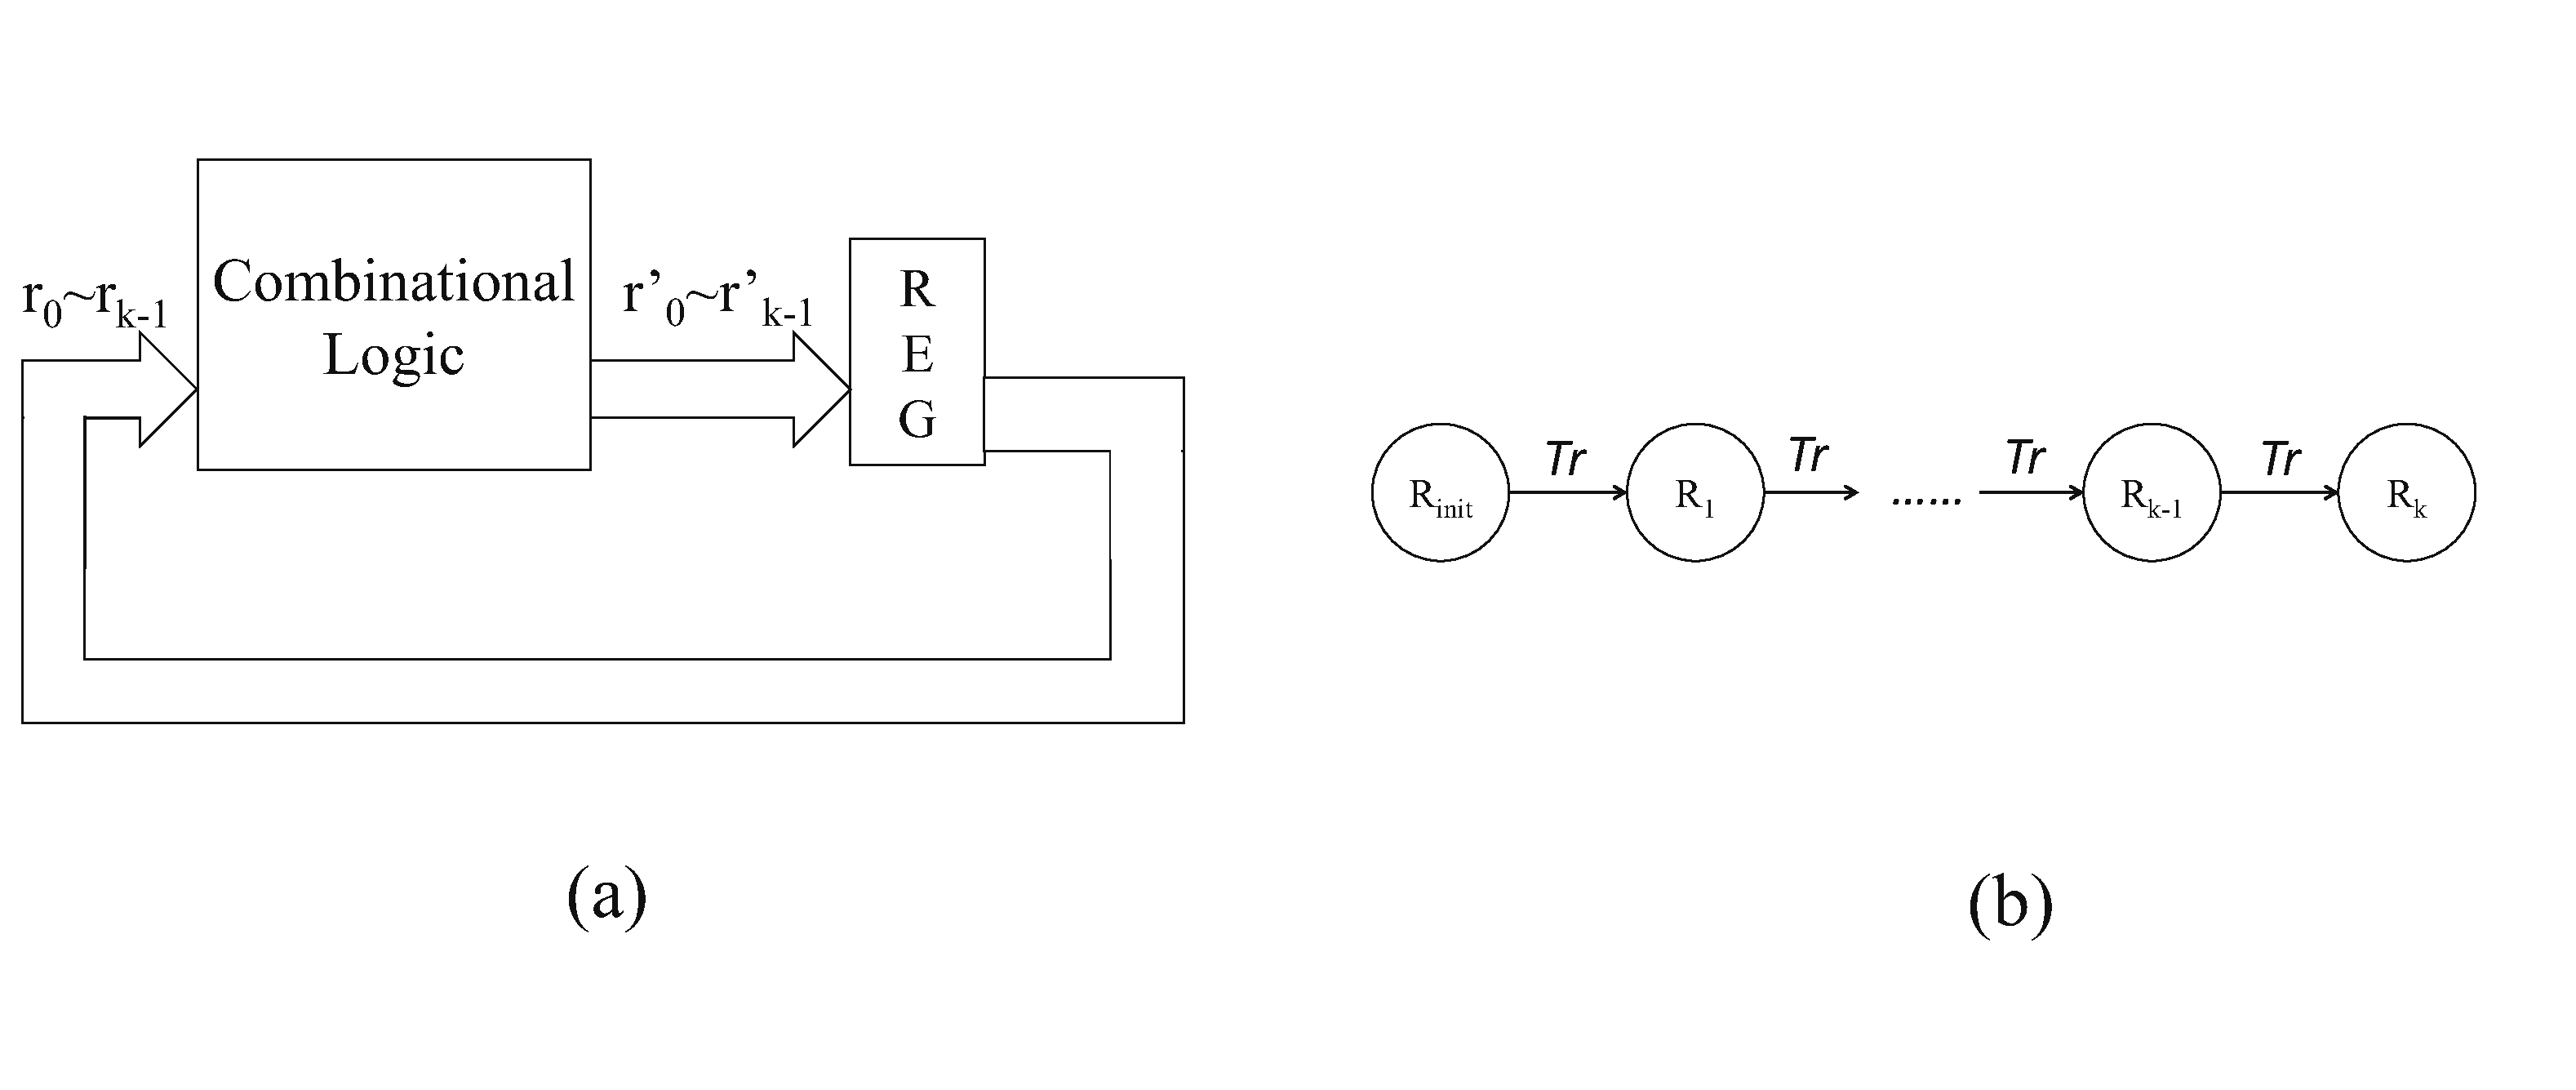
\includegraphics[width=7.5in]{./Moore.eps}
% % \vspace{-0.2in}
% \caption{A simple Moore FSM and its state transition graph}
% %\end{minipage}
% \label{fig:Moore}}
% \end{figure}

Fig.\ref{fig:seqmodel}(b) shows a typical Moore FSM without primary inputs, $R$ is the word-level state variable. Let word-level indeterminate 
$R_{init}$ denote the initial preloaded value of $R$, and $R_{i}$ denote the evaluation of $R$ after $i$ clock cycles
(transitions). Transition relation $Tr:R_{i-1}\to R_i$ can be modeled similar to
the image function in Algorithm \ref{alg:BFS}. Assume that after $k$ clock cycles, the machine should give a state output
$R_{k} = \mathcal F(R_{init})$. To verify this result, we can implicitly unroll this FSM and execute transition
function at word level for $k$ times, which is $R_{k} = Tr(R_{k-1}) = Tr(Tr(\cdots Tr(R_{init})\cdots)) = Tr^k(R_{init})$.

Sequential Galois field (GF) multiplier is a typical sequential arithmetic component widely used in cryptographic systems.
Since there is no primary input in the design, it can be regarded as Moore FSM (Fig.\ref{fig:RHmulti}(a))
where $R = \sum_{i=0}^{k-1} r_i \beta^{2^{i}}, ~A = \sum_{i=0}^{k-1} a_i
 \beta^{2^{i}}, ~B = \sum_{i=0}^{k-1} b_i \beta^{2^{i}}$. Notice that $\beta$ is the {\it normal element}
 which can be represented by a power of primitive element $\alpha:~\beta = \alpha^t$.
The states are encoded by evaluations of state variables, which can be implicitly verified 
by checking output-input function ($R = A\cdot B \pmod{P(\alpha)}$). 

% Additionally
% the inner structure of GF multiplier is XOR-rich such that we can test our approach on very large
% (>100 bits datapath) circuits.
% 
% Let us briefly describe the fundamentals behind the design of normal
% basis sequential GF multipliers, so as to put in perspective the type
% of designs that have been verified in this paper. Let $R =
% \sum_{i=0}^{k-1} r_i \beta^{2^{i}}, ~A = \sum_{i=0}^{k-1} a_i
% \beta^{2^{i}}, ~B = \sum_{i=0}^{k-1} b_i \beta^{2^{i}}$, then 
% \[
% R = A\cdot B = (\sum_{i=0}^{k-1} a_i \beta^{2^{i}}) (\sum_{j=0}^{k-1}
% b_j \beta^{2^{j}})  =
% \sum_{i=0}^{k-1}\sum_{j=0}^{k-1}a_ib_j\beta^{2^i}\beta^{2^j}\nonumber 
% \]
% 
% The expressions $\beta^{2^i}\beta^{2^j}$ are called cross-product
% terms and they can also be represented in normal basis: 
% \begin{displaymath}
% \beta^{2^i}\beta^{2^j} =
% \sum_{n=0}^{k-1}\lambda_{ij}^{(n)}\beta^{2^n}, \ \ \lambda_{ij}^{(n)}
% \in \Ftwo. 
% \end{displaymath}
% 
% From the above two equations, one can see that the expression for the
% $n^{th}$ digit of product $R = (r_0, \dots, r_n, \dots r_{k-1})$ is:
% \[
% r_n = \sum_{i=0}^{k-1}\sum_{j=0}^{k-1}\lambda_{ij}^{(n)}a_ib_j = A
% \cdot M_n \cdot B^T, ~~0 \leq n \leq k-1
% \]
% 
% where $M_n = (\lambda_{ij}^{(n)})$ is a binary $k \times k$ matrix over
% $\Ftwo$, and it is called the $\lambda$-matrix. 
%The collection of all
%$\{M_n\}$  $\lambda$-matrices is called the multiplication
%table. 
% Moreover, let $r_n = A \cdot M_n \cdot B^T$.
% Then $r_{n-1} = A \cdot M_{n-1} \cdot B^T = rotate(A) \cdot M_n
% \cdot rotate(B)^T$. This implies that $M_n$ is generated by right
% and down cyclic shifting $M_{n-1}$. Therefore, the hardware design
% of sequential GF multipliers is based on mappings of $A\cdot M_n
% \cdot B^T$ into AND-XOR gates and cyclic shift operations. 

% This paper verifies the implementation of two distinct 
% architectures of {\it sequential multipliers with parallel output
%   (SMPO)}, namely: i) the Agnew-SMPO  \cite{agnew1991implementation}
% by G. B. Agnew, which is a straight-forward implementation of the
% $\lambda$-matrix; and ii) the more recent, more complicated, yet very
% efficient RH-SMPO \cite{RHmulti}, by Reyhani-Masoleh and Hasan,
% depicted in Fig. \ref{fig:RHmulti}.  

In this proposal we use the verification of a sequential GF multiplier -- 
a 3-bit RH-SMPO invented by Reyhani-Masoleh and Hasan\cite{RHmulti} -- to illustrate our approach.
The normal element is given as $\beta = \alpha^3$, and primitive polynomial $P(\alpha) = \alpha^3+\alpha+1$.
The gate-level circuit is depicted in Fig.\ref{fig:RHmulti}(b).

\begin{figure}[hbt]
\centering{
%\begin{minipage}{12cm}
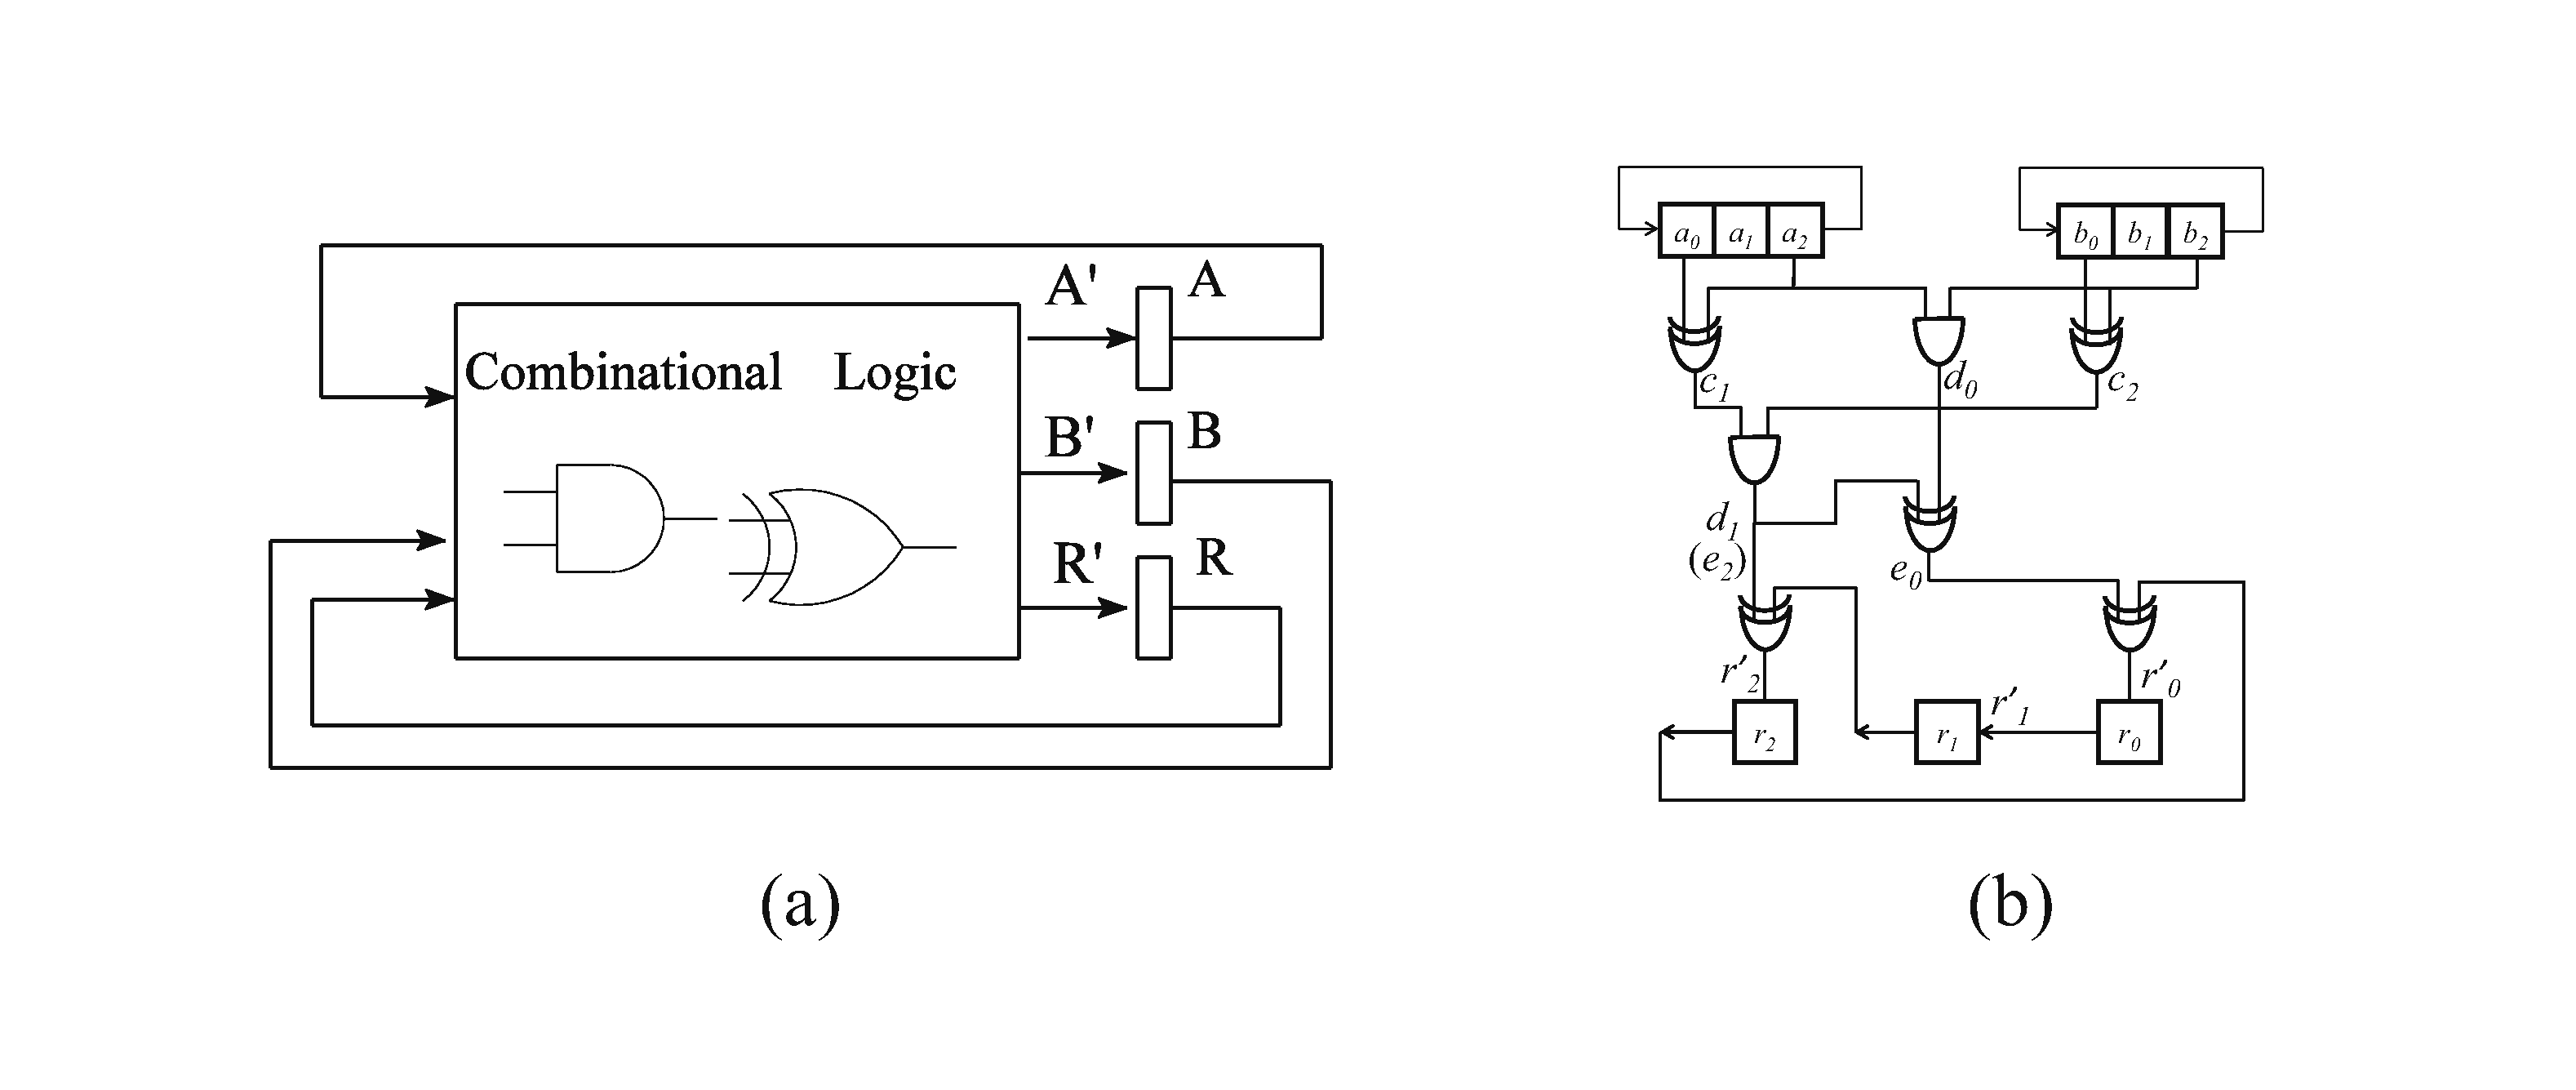
\includegraphics[width=7.5in]{./new_multi.eps}
% \vspace{-0.2in}
\caption{A 3-bit RH-SMPO and its Moore FSM model}
%\end{minipage}
\label{fig:RHmulti}}
\end{figure}

We follow  the typical sequential GF circuit model with word-level variables $A, B, R$
denoting {\it present states (PS)} and $A', B', R'$ denoting {\it next
  states (NS)} of the machine; where $A = \sum_{i=0}^{k-1} a_i \beta^{2^i}$
for the PS variables and $A' = \sum_{i=0}^{k-1} a_i'
\beta^{2^i}$ for NS variables, and so on.  Variables $R\ (R')$ correspond to those that 
store the result, and $A, B\ (A', B')$ store input operands. {\it E.g.,}
for a GF multiplier, $A_{init}, B_{init}$ (and $R_{init} =
0$) are the initial values (operands) loaded into the registers,  and
$R = \F(A_{init}, B_{init}) = A_{init} \times B_{init}$ is the final
result after $k$-cycles. Our approach aims to find this polynomial
representation for $R$.  

Each gate in the combinational logic is represented by a Boolean
polynomial. To 
this set of Boolean polynomials, we append the polynomials that define
the word-level to bit-level relations for PS and NS variables ($A =
\sum_{i=0}^{k-1} a_i \beta^{2^i}$). We denote this set of polynomials
as ideal $J = \langle 
f_1, \dots, f_s \rangle \subset \Fkk[x_1, \dots, x_d, R, R', A, A', B,
  B']$, where $x_1, \dots, x_d$ denote the bit-level (Boolean) variables
  of the circuit. The ideal of vanishing polynomials $J_0$ is also included, and
then the implicit FSM unrolling problem is setup for abstraction. 

The configurations of the flip-flops are the states of the
machine. {\it Since the set of states is a finite set of points, we
can consider it as the variety of an ideal related to the circuit
}. Moreover, since we are interested in
the {\it function encoded} by the state variables (over $k$-time
frames), we can {\it project this variety} on the word-level state
variables, starting from the initial state $A_{init}, B_{init}$.
Projection of varieties (geometry) corresponds to elimination ideals
(algebra), and can be analyzed via \Grobner bases. Therefore, we
employ a \Grobner basis computation with abstraction term order (ATO)\cite{timDAC}: we use a {\it lex term
  order} with {\it bit-level variables} 
$>$ {\it word-level NS outputs} $>$ {\it word-level PS inputs}. This
allows to eliminate all the bit-level variables 
%(corresponding to the combinational logic and the state variables),
%so as to 
and derives a representation only in terms of words. 
Consequently, $k$-successive \Grobner basis computations implicitly
unroll the machine, and provide word-level algebraic $k$-cycle
abstraction for $R'$ as $R' = \F(A_{init}, B_{init})$. 

Algorithm
\ref{alg:modified} describes our approach.  In the algorithm, $from_i$
and $to_i$ are polynomial ideals whose varieties are the valuations of
word-level variables $R, A, B$ and $R',A',B'$ in the $i$-th iteration;
and the notation ``$\setminus$'' signifies that the $NS$ in iteration
$(i)$ becomes the $PS$ in iteration $(i+1)$. Line 5 computes the Gr\"obner 
basis with the abstraction term order.  Line 6 computes the elimination 
ideal, eliminating the bit-level variables and representing the set of 
reachable states up to iteration $i$ in terms of the elimination ideal. 
These computations are analogous to those of image computations performed in FSM reachability. 
%The forward image
%$to^{i}$ is computed using \Grobner bases with ATO.

\vspace{-0.1in}
\IncMargin{1em}
\begin{algorithm}[hbt]
\SetAlgoNoLine
\LinesNumbered
 \KwIn{Circuit polynomial ideal $J$, vanishing ideal $J_0$, initial
   state ideal $R (=0), \mathcal{G}(A_{init}), \mathcal{H}(B_{init})$} 

  $from_0(R,A,B) = \langle R, \mathcal{G}(A_{init}), \mathcal{H}(B_{init})\rangle$\;
  $i = 0$\;
  \Repeat{$i == k$}
  {
  	$i \gets i + 1$\;
%	$to^i(R',A',B') \gets$  $GB( \langle J_{ckt}, J_0,
%    from^{i-1}(R,A,B)\rangle )$ with abstraction term order\;
	$G \gets$GB$( \langle J + J_0+ from_{i-1}(R,A,B) \rangle
    )$ with ATO\;
	$to_i(R',A',B')\gets G\cap \mathbb F_{2^k}[R',A',B',R,A,B]$\;
	$from_i \gets to_i(\{R,A,B\}\setminus \{R',A',B'\})$\;
  }
\Return{$from_k(R_{final})$}
\caption {Abstraction via implicit unrolling for Sequential GF circuit
  verification}
\label{alg:modified}
\end{algorithm}
\DecMargin{1em}
\vspace{-0.1in}
\begin{Example}
\label{ex:RHSMPO}

We demonstrate our approach to verify the 3-bit RH-SMPO circuit of
Fig.\ref{fig:RHmulti}. The normal element $\beta$ in
$\mathbb{F}_{2^3}$ is known to be $\beta = \alpha^3$, where $\alpha$
is the primitive element. The circuit can be described with an ideal by translating
AND and XOR gates accordingly. For the first iteration:
\begin{align*}
J = &d_0+b_2\cdot a_2,
c_1+a_0+a_2,
c_2+b_0+b_2,
d_1+c_1\cdot c_2,\\
&e_0+d_0+d_1,
e_2+d_1,
r_0'+r_2+e_0,
r_1'+r_0,
r_2'+r_1+e_2,\\
&A+a_0\alpha^3+a_1\alpha^6+a_2\alpha^{12},
B+b_0\alpha^3+b_1\alpha^6+b_2\alpha^{12},\\
&R+r_0\alpha^3+r_1\alpha^6+r_2\alpha^{12},
R'+r_0'\alpha^3+r_1'\alpha^6+r_2'\alpha^{12};
\end{align*}
The last 4 polynomials are translated from the definition of word-level variables.
This represents ideal ``$J$" from line 5 in Algorithm
\ref{alg:modified}. ``$J_0$" is the ideal of vanishing polynomials in all bit-level
variables (e.g. $a_0^2-a_0$) and word-level variables (e.g. $A^8-A$). ``$from_{i-1}$"
represents the set of current states for iteration $i$.
In the first iteration, $from_0 = \{R, A_{init}+a_0\alpha^3+a_1\alpha^6+a_2\alpha^{12},
B_{init}+b_0\alpha^3+b_1\alpha^6+b_2\alpha^{12}\}$.

After the GB computation is performed with ATO, as line 6 in Algorithm \ref{alg:modified},
we find a polynomial in variables $R', A_{init}, B_{init}$ in $to_1 : 
R'+(\alpha^2) A_{init}^4 B_{init}^4+(\alpha^2+\alpha) A_{init}^4 B_{init}^2+(\alpha^2+\alpha) A_{init}^4 B_{init}+(\alpha^2+\alpha) A_{init}^2 B_{init}^4+(\alpha^2+\alpha+1) A_{init}^2 B_{init}^2+(\alpha^2) A_{init}^2 B_{init}+(\alpha^2+\alpha) A_{init} B_{init}^4+(\alpha^2) A_{init} B_{init}^2
$.

Line 7 in Algorithm \ref{alg:modified} simply replaces NS output $R'$ with PS output
$R$ in this example; so in second iteration $from_1 = \{
R'+(\alpha^2) A_{init}^4 B_{init}^4+(\alpha^2+\alpha) A_{init}^4 B_{init}^2+(\alpha^2+\alpha) A_{init}^4 B_{init}+(\alpha^2+\alpha) A_{init}^2 B_{init}^4+(\alpha^2+\alpha+1) A_{init}^2 B_{init}^2+(\alpha^2) A_{init}^2 B_{init}+(\alpha^2+\alpha) A_{init} B_{init}^4+(\alpha^2) A_{init} B_{init}^2
, A_{init}+a_2\alpha^3+a_0\alpha^6+a_1\alpha^{12},
B_{init}+b_2\alpha^3+b_0\alpha^6+b_1\alpha^{12}\}$. 

% By continue executing the loop,
Finally, after 3 iterations we obtain: $to_3 = \{ \mathbf{R'+A_{init}B_{init},}
~A_{init}+a_0'\alpha^3+a_1'\alpha^6+a_2'\alpha^{12},
~B_{init}+b_0'\alpha^3+b_1'\alpha^6+b_2'\alpha^{12}\}$
as the image. The final result is $from_3(R_{final}) = R_{final}+A_{init}\cdot
B_{init}$, which verifies the multiplier. 
\end{Example}
Using our approach we successfully verified the function of an 100-bit RH-multiplier,
which implies its capability to handle the verification of large designs. The results
are published in \cite{myDATE}.
\section{Refined Algorithm}
Within the naive algorithm described in last section, Gr\"obner basis is computed for each
iteration to attain the word-level next state polynomial representation. In practice, for 
a sequential circuit with complicated structure and large datapath, Gr\"obner basis computation
is intractable. To overcome the high computational complexity brought by GB computing, 
we managed to find a method obviating directly computing GB; more specifically, we turn 
GB computation into one-step multivariate polynomial division. In this way, our proposed 
approach can be used on larger sequential circuit verification.


\subsection{Refined abstraction term order (RATO)}
A lexicographic order constrained by following relation $>_{r}$: "circuit variables ordered reverse topologically" $>$ 
"designated word-level output" $>$ "word-level inputs" is called the \emph{Refined Abstraction Term Order (RATO)}.

In Buchberger's algorithm, the specification polynomial (Spoly) for each pair is calculated. In RATO, most polynomials
have relatively prime leading terms/monomials (which means $Spoly \xrightarrow{J+J_0}_{+} 0$) except one pair:
word-level polynomial corresponding to outputs and its leading bit-level variable's gate description polynomial.
Its remainder $r$ lets following lemma hold:

\begin{Lemma}
\label{lem:1}
$r$ will only contain primary inputs (bit-level) and word-level output; furthermore, there will be one and
only one term containing word-level output whose monomial is word-level output itself rather than higher order form.
\end{Lemma}

\begin{proof}
First proposition is easy to prove by contradiction. Second part, the candidate pair of polynomials only have one term of
single word-level output variable (say it is $R$) and this term is the last term under RATO, which means there is only one term with
$R$ in Spoly. Meanwhile in other polynomials from $J+J_0$ there is no such term containing $R$, so this term will be
kept to remainder $r$, in first degree.
\end{proof}

\begin{Example}
After adding intermediate bit-level signal $a,b,c,d$, the elimination ideal for example circuit (Ex.\ref{ex:SMPO}) 
could be rewritten under RATO:
\begin{align}
&(t_0,t_1)>(a,b,c,d)\nonumber\\&>T>(x,s_0,s_1)\nonumber
\end{align}
Thus the candidate pair is
$(f_w,f_g), f_w = t_0+a\cdot b+a+b, f_g =t_0+t_1\alpha + T$.
Result after reduction is:
\begin{align}
&Spoly(f_w,f_g) \xrightarrow{J+J_0}_{+}\nonumber\\
&T + s_0 s_1 x+s_0 s_1 \alpha+(1+\alpha)s_0 x+(1+\alpha) s_0+s_1 x+s_1+(1+\alpha) x+1\nonumber
\end{align}
The remainder satisfies Lemma \ref{lem:1}.
\end{Example}

\subsection{Bit-level Variable Substitution (BLVS)}
\label{sec:blvs}
The remainder from \emph{Spoly} contains bit-level PS variables, and our objective is to get a polynomial contains only word-level PS variables
. One possible method is to rewrite bit-level variables in term of function on word-level
variables, i.e.
\begin{equation}
\label{eqn:BLVS}
s_i = \mathcal{G}(S)
\end{equation}
then do substitution. One way to obtain Eqn.\ref{eqn:BLVS} is to apply a Gaussian-elimination-fashion approach, which could 
compute corresponding $\mathcal{G}(S)$ efficiently with time complexity $O(k^3)$.

\begin{Example}
{\bf Objective}:\ Abstract polynomial $s_i + \mathcal{G}_i(S)$ from $f_0: s_0+s_1\alpha+S$.

First, compute $f_0^2: s_0+s_1\alpha^2+S^2$. Apparently variable $s_0$ can be
eliminated by operation 
\begin{align}
f_1 =& f_0 + f_0^2: \nonumber\\
&(\alpha^2+\alpha)s_1+S^2+S\nonumber
\end{align}
Now we can solve univariate polynomial equation $f_1 = 0$ and get solution
$$s_1 = S^2 + S$$
Use this solution we can easily solve equation $f_0 = 0$. The result is
$$s_0 = \alpha S^2+(1+\alpha)S$$
\end{Example}

Another formalized method is to solve following system of equations
\begin{align}
\label{eqn:betamat}
\begin{bmatrix}
S \\
S^2 \\
S^{2^2} \\
\vdots \\
S^{2^{k-1}}
\end{bmatrix}
&=
\begin{bmatrix}
\beta & \beta^{2} & \beta^{2^2} & \cdots & \beta^{2^{k-1}}\\
\beta^{2} & \beta^{2^2} & \beta^{2^3} & \cdots & \beta \\
\beta^{2^2} & \beta^{2^3} & \beta^{2^4} & \cdots & \beta^2\\
\vdots & \vdots & \vdots & \ddots & \vdots \\
\beta^{2^{k-1}} & \beta & \beta^2 & \cdots & \beta^{2^{k-2}}
\end{bmatrix}
\begin{bmatrix}
s_0\\
s_1\\
s_2\\
\vdots\\
s_{k-1}
\end{bmatrix}
\end{align}
Let ${\bf s}$ be a vector of $k$ unknowns $s_0,\dots,s_{k-1}$,
then Eqn.\ref{eqn:betamat} can be solved by using Cramer's rule:
\begin{equation}
\label{eqn:Cramer}
s_i = \frac{\Mi}{\M}, \ \ 0\leq i\leq k-1, \M \neq 0
\end{equation}
where ${\bf M_i}$ denotes a coefficient matrix replacing $i$-th column in ${\bf M}$ with
vector ${\bf S} = [S~~S^2~~\cdots~~S^{2^{k-1}}]^T$.

Notice that ${\bf M}$ is constructed by squaring a row and assigning it to next row,
therefore its determinant belongs to a special sort of determinants:
\begin{Definition}
Let $\{\alpha_0,\alpha_1,\dots,\alpha_{k-1}\}$ be a set of $k$ elements of $\Fpk$. Then the determinant
\begin{align}
\det{M(\alpha_0,\dots,\alpha_{k-1})} &= 
\begin{vmatrix}
\alpha_0 & \alpha_1 & \cdots & \alpha_{k-1} \\
\alpha_0^p & \alpha_1^p & \cdots & \alpha_{k-1}^p \\
\vdots & \vdots & \ddots & \vdots \\
\alpha_0^{p^{k-1}} & \alpha_1^{p^{k-1}} & \cdots & \alpha_{k-1}^{p^{k-1}}
\end{vmatrix}
\end{align}
is called the {\bf Moore determinant} of set $\{\alpha_0,\dots,\alpha_{k-1}\}$.
\end{Definition}
Moore determinant can be written as an explicit expression
\begin{equation}
\label{eqn:Moore}
\det{M(\alpha_0,\dots,\alpha_{k-1})} = \alpha_0 \prod_{i=1}^{k-1} \prod_{c_0,\dots,c_{i-1}\in \Fp} (\alpha_{i} - \sum_{j=0}^{i-1}c_j\alpha_j)
\end{equation}
We use an example to help understanding the notations in Eqn.\ref{eqn:Moore}:
\begin{Example}
Let $\{\alpha_0,\alpha_1,\alpha_2\}$ be a set of elements of $\mathbb F_{2^3}$. Then
\begin{align}
\det{M(\alpha_0,\alpha_1,\alpha_2)} &= 
\begin{vmatrix}
\alpha_0 & \alpha_1 & \alpha_2 \\
\alpha_0^2 & \alpha_1^2 & \alpha_2^2 \\
\alpha_0^4 & \alpha_1^4 & \alpha_2^4
\end{vmatrix} \\ \nonumber
=& \alpha_0 \prod_{i=1}^{2} \prod_{c_0,\dots,c_{i-1}\in \Ftwo} (\alpha_{i} - \displaystyle\sum_{j=0}^{i-1}c_j\alpha_j)
\end{align}
First, let $i=1$,  we obtain $c_0\in \Ftwo$. When $c_0=0$, the product term equals to $\alpha_1$; when $c_0=1$ it equals to $(\alpha_1-\alpha_0)$.
Then let $i=2$, we obtain ${c_0,c_1}\in \Ftwo$, they can take value from $\{0,0\},\{0,1\},\{1,0\}$ and $\{1,1\}$.
We add 4 more product terms $\alpha_2,(\alpha_2-\alpha_1),(\alpha_2-\alpha_0),(\alpha_2-\alpha_0-\alpha_1)$ respectively.

Thus, the result is
\begin{equation}
\det{M(\alpha_0,\alpha_1,\alpha_2)} = \alpha_0\alpha_1(\alpha_1-\alpha_0)\alpha_2(\alpha_2-\alpha_1)(\alpha_2-\alpha_0)(\alpha_2-\alpha_0-\alpha_1)
\end{equation}
\end{Example}
We discover through investigation that $\M$ has a special property when the set of elements forms a basis. The proof is given below:
\begin{Lemma}
\label{lemma:Moore}
Let $\{\alpha_0,\alpha_1,\dots,\alpha_{k-1}\}$ be a normal basis of $\Fpk$ over $\Fp$. Then
\begin{equation}
\det{M(\alpha_0,\alpha_1,\dots,\alpha_{k-1})} = 1
\end{equation}
\end{Lemma}
\begin{proof}
According to the definition Eqn.\ref{eqn:Moore}, the Moore determinant consists of all possible linear combinations of 
$\{\alpha_0,\alpha_1,\dots,\alpha_{k-1}\}$ with coefficients over $\Fp$. If $\{\alpha_0,\alpha_1,\dots,\alpha_{k-1}\}$
is a (normal) basis, then all product terms are distinct and represents all elements in the field $\Fpk$. Since the product 
of all elements of a field equals to 1, the Moore determinant $\M=1$.
\end{proof}
Applying Lemma \ref{lemma:Moore} to Eqn.\ref{eqn:Cramer} gives
\begin{equation}
s_i = \Mi,~~0\leq i\leq k-1
\end{equation}
where $\Mi$ can be easily computed using Laplace expansion method, with complexity $O(k!)$.

In this approach it is easy to get word-level variable representation for each bit-level PS variables. 
By substitution, a new polynomial in word-level PS/NS variables could be attained.

After processing with RATO and BLVS techniques, we get a polynomial in form of $f_T = T+\mathcal{F}(S,x)$
denoting the transition function. We add a polynomial about $S$ to define the present states $f_S$,
as well as a polynomial guarantee free-end signals for primary inputs $f_x = x^2+x$, using elimination term order $S>x>T$,
we can generate a GB out of elimination ideal $\langle f_T,f_S,f_x\rangle$, which contains a univariate
polynomial denoting next states. The new scalable algorithm can be depicted as following:

\begin{algorithm}[hbt]
\SetAlgoNoLine
 \KwIn{Input-output circuit characteristic polynomial ideal $J_{ckt}$, initial state polynomial $\F(S)$}

  $from^0 = reached = \F(S)$\;
  $f_T = $Reduce(spoly$(f_w,f_s), J_{ckt})$\;
  \tcc{Compute S-poly for the critical pair, then reduce it with circuit ideal under RATO}
  \Repeat{$\langle new^i\rangle == \langle 1\rangle$}
  {
  	$i \gets i + 1$\;
  	$G \gets$GB($\langle f_T ,f_x, from^{i-1}\rangle$)\;
  	\tcc{Compute Gr\"obner basis with elimination term order: $T$ smallest; $f_x$ is polynomial covers all possible inputs from PIs}
	$\langle to^i \rangle \gets G\cup \Fkk[T]$\;
	\tcc{There will be a univariate polynomial in $G$ denoting next state in word-level variable $T$}
	$\langle new^i\rangle \gets \langle to^i\rangle + (\langle T^{2^k}-T\rangle:\langle reached\rangle)$\;
	\tcc{Use quotient of ideals to attain complement of reached states, then use sum of ideals to attain an intersection with next state}
  	$\langle reached\rangle \gets \langle reached\rangle \cdot \langle new^i\rangle$\;
  	\tcc{Use product of ideals to attain a union of newly reached states and formerly reached states}
	$from^i \gets new^i(S\setminus T)$\;
	\tcc{Start a new iteration by replacing variable $T$ in newly reached states with current state variable $S$}
  }
  \tcc{Loop until a fixpoint reached: newly reached state is empty}
\Return{$\langle reached\rangle$}
\caption {Refined Algebraic Geometry based Traversal Algorithm}\label{alg:refined}
\end{algorithm}

\subsection{PI Partition}
Using above techniques we can get a remainder polynomial with only word-level PS/NS variables. However in most 
cases, the number of bit-level PIs will be too large for the last-step Gr\"obner basis computation. Therefore it is necessary
to convert bit-level PIs to word-level PI variables. 

Assume we have $k$-bit datapath and $n$-bit PIs. In Galois field, we need to carefully partition $n$ PIs
to guarantee states of all partitions can be covered by single univariate polynomials.

\begin{Proposition}
Divide $n$-bit PIs to partitions $n_1,n_2,\dots, n_s$ and let $n_1,n_2,\dots,n_s$ bit word-level variables
represent their evaluations in $\mathbb F_{2^k}$ accordingly. Then there always be $n_1,n_2,\dots,n_s~|~k$.
\end{Proposition}

Again, assume a partition $n_i~|~k$ and corresponding word-level variable is $P$. Then we can use polynomial
$P^{2^n_i}-P$ to represent all signals at free-end PIs, according to following theorem about {\bf composite
field}:
\begin{Theorem}
\label{thm:composite}
Let $k = m\dot n_i$, such that $\mathbb F_{2^k} = \mathbb F_{(2^{n_i})^m}$. Let $\alpha$ be primitive root of 
$\mathbb F_{2^k}$, $\beta$ be primitive root of the ground field $\mathbb F_{2^{n_i}}$. Then
$$\beta = \alpha^\omega,~~\text{where}~~\omega = \frac{2^k-1}{2^{n_i}-1}$$
\end{Theorem}
\begin{Example}
In a sequential circuit, PS/NS inputs/outputs are 4-bit signals, which means we will use $\mathbb F_{2^4}$
as working field. PIs are partitioned to 2-bit vectors, which means the ground field is $\mathbb F_{2^2}$.
In ground field we can represent all possible evaluations of this PI partition $\{p_0,p_1\}$ with
$$P^4+P,~~\text{where}~~P=p_0+p_1\cdot\beta$$
Using Thm.\ref{thm:composite} we get $\beta = \alpha^5$, so we can redefine word $P$ as element from $\mathbb F_{2^4}$:
$$P = p_0 + p_1\cdot\alpha^5$$
\end{Example}
Using this method we can efficiently partition large size PIs to small number of word-level PI variables.
One limitation of this approach is PIs cannot be partitioned when $k$ is prime.
\section{Application: Unrolling Sequential Circuits for Sequential Arithmetic Verification}
In above discussions, we propose an implicit state enumeration algorithm implemented by GB computations over
an elimination ideal, which is usually applied on FSMs working as control units. For many arithmetic
datapath components, state enumeration is not the best way to verify the function of circuit. On the one hand, the signals preloaded
to the state variables in FSM are usually not specified such that we can hardly encode the initial states; on the other
hand, instead of the set of globally reachable states, arithmetic verification focuses on exact reached states
after $k$ clock cycles which reflects desired arithmetic function. Considering these reasons, we modify
our algebraic geometry based approach and apply it to implicit FSM unrolling. 

% In above discussions, we propose an implicit state enumeration algorithm implemented by GB computation over
% an elimination ideal, which is usually applied on Mealy FSMs working as control unit. For many arithmetic
% datapath components, they should be modeled as Moore FSMs according to their structures. On the one hand, the signals preloaded
% to a Moore FSM are usually not specified such that we can hardly encode the initial states; on the other
% hand, instead of the set of globally reachable states, arithmetic verification focuses on exact reached states
% after $k$ clock cycles which reflects desired arithmetic function. Considering these reasons, we modify
% our algebraic geometry based approach and apply it to Moore FSM unrolling. 

% % Figure Moore.eps
% \begin{figure}[hbt]
% \centering{
% %\begin{minipage}{12cm}
% 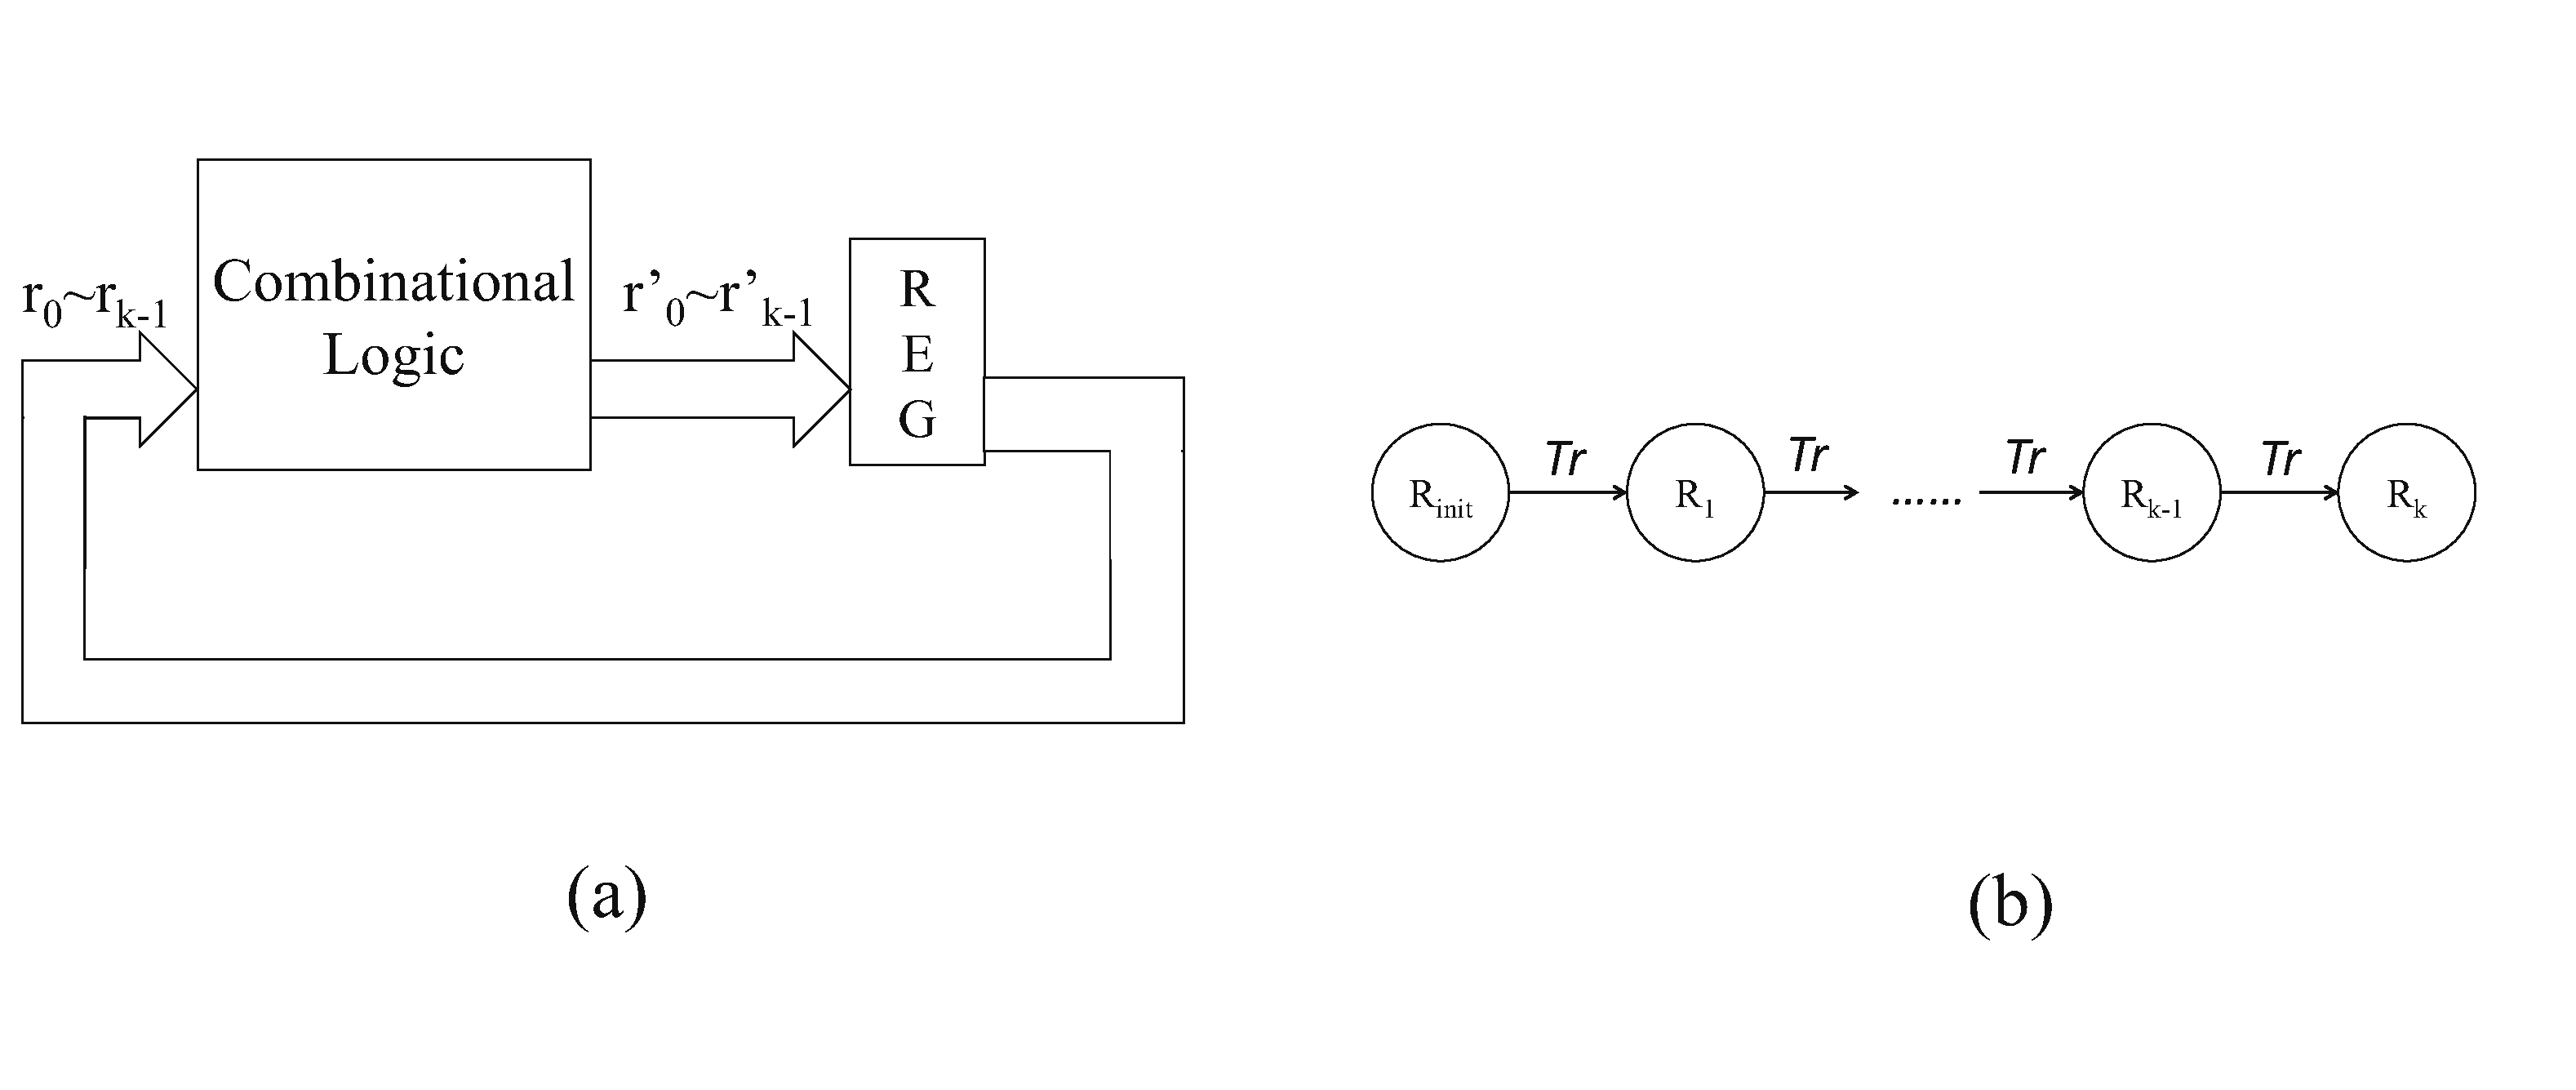
\includegraphics[width=7.5in]{./Moore.eps}
% % \vspace{-0.2in}
% \caption{A simple Moore FSM and its state transition graph}
% %\end{minipage}
% \label{fig:Moore}}
% \end{figure}

Fig.\ref{fig:seqmodel}(b) shows a typical Moore FSM without primary inputs, $R$ is the word-level state variable. Let word-level indeterminate 
$R_{init}$ denote the initial preloaded value of $R$, and $R_{i}$ denote the evaluation of $R$ after $i$ clock cycles
(transitions). Transition relation $Tr:R_{i-1}\to R_i$ can be modeled similar to
the image function in Algorithm \ref{alg:BFS}. Assume that after $k$ clock cycles, the machine should give a state output
$R_{k} = \mathcal F(R_{init})$. To verify this result, we can implicitly unroll this FSM and execute transition
function at word level for $k$ times, which is $R_{k} = Tr(R_{k-1}) = Tr(Tr(\cdots Tr(R_{init})\cdots)) = Tr^k(R_{init})$.

Sequential Galois field (GF) multiplier is a typical sequential arithmetic component widely used in cryptographic systems.
Since there is no primary input in the design, it can be regarded as Moore FSM (Fig.\ref{fig:RHmulti}(a))
where $R = \sum_{i=0}^{k-1} r_i \beta^{2^{i}}, ~A = \sum_{i=0}^{k-1} a_i
 \beta^{2^{i}}, ~B = \sum_{i=0}^{k-1} b_i \beta^{2^{i}}$. Notice that $\beta$ is the {\it normal element}
 which can be represented by a power of primitive element $\alpha:~\beta = \alpha^t$.
The states are encoded by evaluations of state variables, which can be implicitly verified 
by checking output-input function ($R = A\cdot B \pmod{P(\alpha)}$). 

% Additionally
% the inner structure of GF multiplier is XOR-rich such that we can test our approach on very large
% (>100 bits datapath) circuits.
% 
% Let us briefly describe the fundamentals behind the design of normal
% basis sequential GF multipliers, so as to put in perspective the type
% of designs that have been verified in this paper. Let $R =
% \sum_{i=0}^{k-1} r_i \beta^{2^{i}}, ~A = \sum_{i=0}^{k-1} a_i
% \beta^{2^{i}}, ~B = \sum_{i=0}^{k-1} b_i \beta^{2^{i}}$, then 
% \[
% R = A\cdot B = (\sum_{i=0}^{k-1} a_i \beta^{2^{i}}) (\sum_{j=0}^{k-1}
% b_j \beta^{2^{j}})  =
% \sum_{i=0}^{k-1}\sum_{j=0}^{k-1}a_ib_j\beta^{2^i}\beta^{2^j}\nonumber 
% \]
% 
% The expressions $\beta^{2^i}\beta^{2^j}$ are called cross-product
% terms and they can also be represented in normal basis: 
% \begin{displaymath}
% \beta^{2^i}\beta^{2^j} =
% \sum_{n=0}^{k-1}\lambda_{ij}^{(n)}\beta^{2^n}, \ \ \lambda_{ij}^{(n)}
% \in \Ftwo. 
% \end{displaymath}
% 
% From the above two equations, one can see that the expression for the
% $n^{th}$ digit of product $R = (r_0, \dots, r_n, \dots r_{k-1})$ is:
% \[
% r_n = \sum_{i=0}^{k-1}\sum_{j=0}^{k-1}\lambda_{ij}^{(n)}a_ib_j = A
% \cdot M_n \cdot B^T, ~~0 \leq n \leq k-1
% \]
% 
% where $M_n = (\lambda_{ij}^{(n)})$ is a binary $k \times k$ matrix over
% $\Ftwo$, and it is called the $\lambda$-matrix. 
%The collection of all
%$\{M_n\}$  $\lambda$-matrices is called the multiplication
%table. 
% Moreover, let $r_n = A \cdot M_n \cdot B^T$.
% Then $r_{n-1} = A \cdot M_{n-1} \cdot B^T = rotate(A) \cdot M_n
% \cdot rotate(B)^T$. This implies that $M_n$ is generated by right
% and down cyclic shifting $M_{n-1}$. Therefore, the hardware design
% of sequential GF multipliers is based on mappings of $A\cdot M_n
% \cdot B^T$ into AND-XOR gates and cyclic shift operations. 

% This paper verifies the implementation of two distinct 
% architectures of {\it sequential multipliers with parallel output
%   (SMPO)}, namely: i) the Agnew-SMPO  \cite{agnew1991implementation}
% by G. B. Agnew, which is a straight-forward implementation of the
% $\lambda$-matrix; and ii) the more recent, more complicated, yet very
% efficient RH-SMPO \cite{RHmulti}, by Reyhani-Masoleh and Hasan,
% depicted in Fig. \ref{fig:RHmulti}.  

In this proposal we use the verification of a sequential GF multiplier -- 
a 3-bit RH-SMPO invented by Reyhani-Masoleh and Hasan\cite{RHmulti} -- to illustrate our approach.
The normal element is given as $\beta = \alpha^3$, and primitive polynomial $P(\alpha) = \alpha^3+\alpha+1$.
The gate-level circuit is depicted in Fig.\ref{fig:RHmulti}(b).

\begin{figure}[hbt]
\centering{
%\begin{minipage}{12cm}
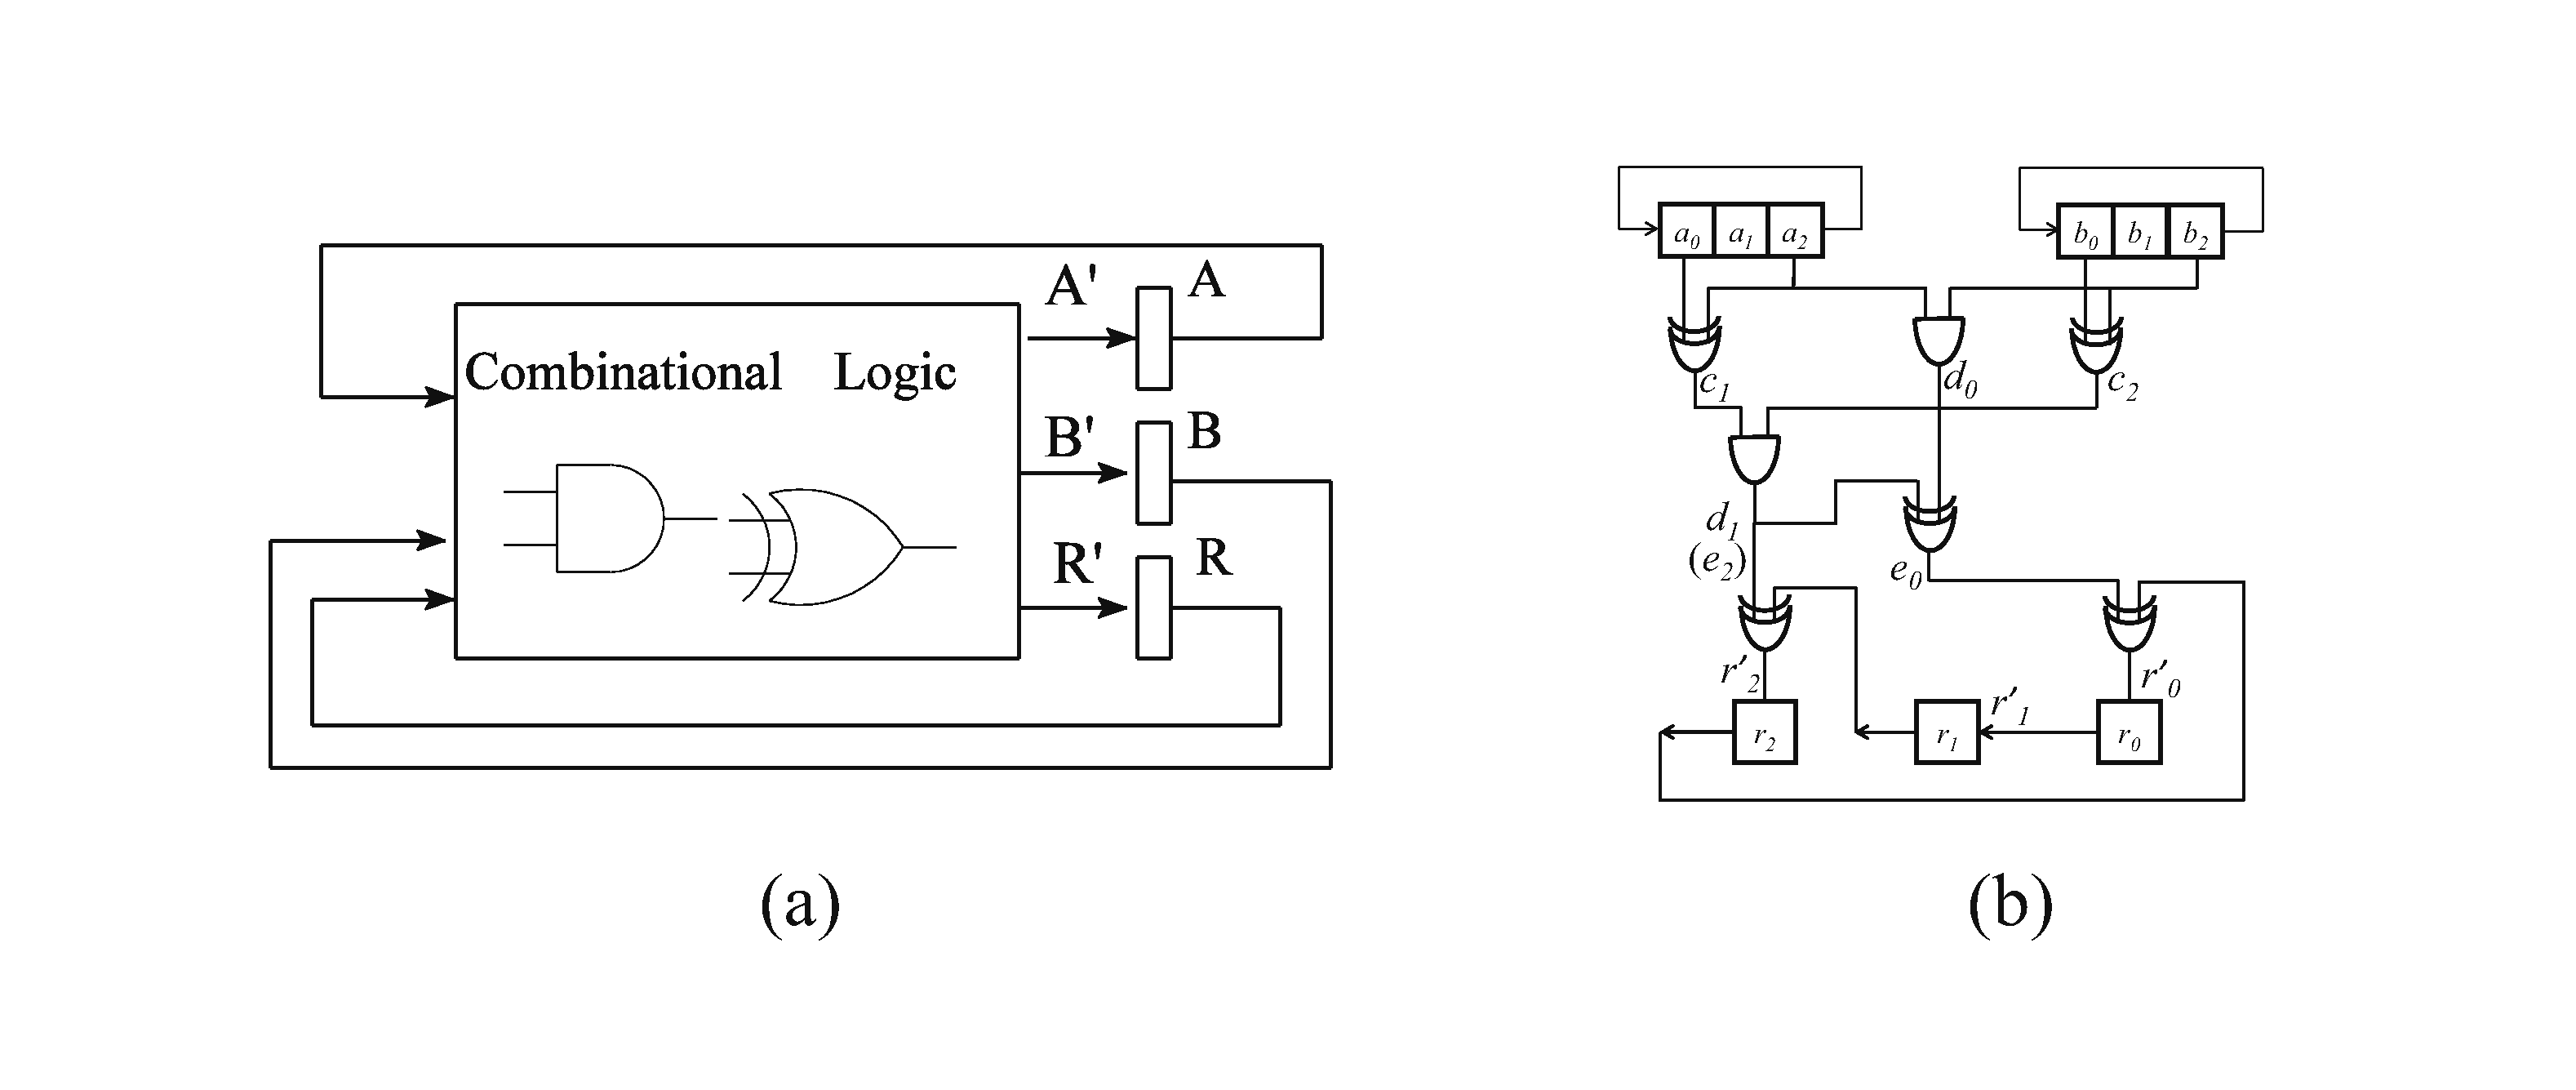
\includegraphics[width=4.5in]{./new_multi.eps}
% \vspace{-0.2in}
\caption{A 3-bit RH-SMPO and its Moore FSM model}
%\end{minipage}
\label{fig:RHmulti}}
\end{figure}

We follow  the typical sequential GF circuit model with word-level variables $A, B, R$
denoting {\it present states (PS)} and $A', B', R'$ denoting {\it next
  states (NS)} of the machine; where $A = \sum_{i=0}^{k-1} a_i \beta^{2^i}$
for the PS variables and $A' = \sum_{i=0}^{k-1} a_i'
\beta^{2^i}$ for NS variables, and so on.  Variables $R\ (R')$ correspond to those that 
store the result, and $A, B\ (A', B')$ store input operands. {\it E.g.,}
for a GF multiplier, $A_{init}, B_{init}$ (and $R_{init} =
0$) are the initial values (operands) loaded into the registers,  and
$R = \F(A_{init}, B_{init}) = A_{init} \times B_{init}$ is the final
result after $k$-cycles. Our approach aims to find this polynomial
representation for $R$.  

Each gate in the combinational logic is represented by a Boolean
polynomial. To 
this set of Boolean polynomials, we append the polynomials that define
the word-level to bit-level relations for PS and NS variables ($A =
\sum_{i=0}^{k-1} a_i \beta^{2^i}$). We denote this set of polynomials
as ideal $J = \langle 
f_1, \dots, f_s \rangle \subset \Fkk[x_1, \dots, x_d, R, R', A, A', B,
  B']$, where $x_1, \dots, x_d$ denote the bit-level (Boolean) variables
  of the circuit. The ideal of vanishing polynomials $J_0$ is also included, and
then the implicit FSM unrolling problem is setup for abstraction. 

The configurations of the flip-flops are the states of the
machine. {\it Since the set of states is a finite set of points, we
can consider it as the variety of an ideal related to the circuit
}. Moreover, since we are interested in
the {\it function encoded} by the state variables (over $k$-time
frames), we can {\it project this variety} on the word-level state
variables, starting from the initial state $A_{init}, B_{init}$.
Projection of varieties (geometry) corresponds to elimination ideals
(algebra), and can be analyzed via \Grobner bases. Therefore, we
employ a \Grobner basis computation with abstraction term order (ATO)\cite{timDAC}: we use a {\it lex term
  order} with {\it bit-level variables} 
$>$ {\it word-level NS outputs} $>$ {\it word-level PS inputs}. This
allows to eliminate all the bit-level variables 
%(corresponding to the combinational logic and the state variables),
%so as to 
and derives a representation only in terms of words. 
Consequently, $k$-successive \Grobner basis computations implicitly
unroll the machine, and provide word-level algebraic $k$-cycle
abstraction for $R'$ as $R' = \F(A_{init}, B_{init})$. 

Algorithm
\ref{alg:modified} describes our approach.  In the algorithm, $from_i$
and $to_i$ are polynomial ideals whose varieties are the valuations of
word-level variables $R, A, B$ and $R',A',B'$ in the $i$-th iteration;
and the notation ``$\setminus$'' signifies that the $NS$ in iteration
$(i)$ becomes the $PS$ in iteration $(i+1)$. Line 5 computes the Gr\"obner 
basis with the abstraction term order.  Line 6 computes the elimination 
ideal, eliminating the bit-level variables and representing the set of 
reachable states up to iteration $i$ in terms of the elimination ideal. 
These computations are analogous to those of image computations performed in FSM reachability. 
%The forward image
%$to^{i}$ is computed using \Grobner bases with ATO.

\vspace{-0.1in}
\IncMargin{1em}
\begin{algorithm}[hbt]
\SetAlgoNoLine
\LinesNumbered
 \KwIn{Circuit polynomial ideal $J$, vanishing ideal $J_0$, initial
   state ideal $R (=0), \mathcal{G}(A_{init}), \mathcal{H}(B_{init})$} 

  $from_0(R,A,B) = \langle R, \mathcal{G}(A_{init}), \mathcal{H}(B_{init})\rangle$\;
  $i = 0$\;
  \Repeat{$i == k$}
  {
  	$i \gets i + 1$\;
%	$to^i(R',A',B') \gets$  $GB( \langle J_{ckt}, J_0,
%    from^{i-1}(R,A,B)\rangle )$ with abstraction term order\;
	$G \gets$GB$( \langle J + J_0+ from_{i-1}(R,A,B) \rangle
    )$ with ATO\;
	$to_i(R',A',B')\gets G\cap \mathbb F_{2^k}[R',A',B',R,A,B]$\;
	$from_i \gets to_i(\{R,A,B\}\setminus \{R',A',B'\})$\;
  }
\Return{$from_k(R_{final})$}
\caption {Abstraction via implicit unrolling for Sequential GF circuit
  verification}
\label{alg:modified}
\end{algorithm}
\DecMargin{1em}
\vspace{-0.1in}
\begin{Example}
\label{ex:RHSMPO}

We demonstrate our approach to verify the 3-bit RH-SMPO circuit of
Fig.\ref{fig:RHmulti}. The normal element $\beta$ in
$\mathbb{F}_{2^3}$ is known to be $\beta = \alpha^3$, where $\alpha$
is the primitive element. The circuit can be described with an ideal by translating
AND and XOR gates accordingly. For the first iteration:
\begin{align*}
J = &d_0+b_2\cdot a_2,
c_1+a_0+a_2,
c_2+b_0+b_2,
d_1+c_1\cdot c_2,\\
&e_0+d_0+d_1,
e_2+d_1,
r_0'+r_2+e_0,
r_1'+r_0,
r_2'+r_1+e_2,\\
&A+a_0\alpha^3+a_1\alpha^6+a_2\alpha^{12},
B+b_0\alpha^3+b_1\alpha^6+b_2\alpha^{12},\\
&R+r_0\alpha^3+r_1\alpha^6+r_2\alpha^{12},
R'+r_0'\alpha^3+r_1'\alpha^6+r_2'\alpha^{12};
\end{align*}
The last 4 polynomials are translated from the definition of word-level variables.
This represents ideal ``$J$" from line 5 in Algorithm
\ref{alg:modified}. ``$J_0$" is the ideal of vanishing polynomials in all bit-level
variables (e.g. $a_0^2-a_0$) and word-level variables (e.g. $A^8-A$). ``$from_{i-1}$"
represents the set of current states for iteration $i$.
In the first iteration, $from_0 = \{R, A_{init}+a_0\alpha^3+a_1\alpha^6+a_2\alpha^{12},
B_{init}+b_0\alpha^3+b_1\alpha^6+b_2\alpha^{12}\}$.

After the GB computation is performed with ATO, as line 6 in Algorithm \ref{alg:modified},
we find a polynomial in variables $R', A_{init}, B_{init}$ in $to_1 : 
R'+(\alpha^2) A_{init}^4 B_{init}^4+(\alpha^2+\alpha) A_{init}^4 B_{init}^2+(\alpha^2+\alpha) A_{init}^4 B_{init}+(\alpha^2+\alpha) A_{init}^2 B_{init}^4+(\alpha^2+\alpha+1) A_{init}^2 B_{init}^2+(\alpha^2) A_{init}^2 B_{init}+(\alpha^2+\alpha) A_{init} B_{init}^4+(\alpha^2) A_{init} B_{init}^2
$.

Line 7 in Algorithm \ref{alg:modified} simply replaces NS output $R'$ with PS output
$R$ in this example; so in second iteration $from_1 = \{
R'+(\alpha^2) A_{init}^4 B_{init}^4+(\alpha^2+\alpha) A_{init}^4 B_{init}^2+(\alpha^2+\alpha) A_{init}^4 B_{init}+(\alpha^2+\alpha) A_{init}^2 B_{init}^4+(\alpha^2+\alpha+1) A_{init}^2 B_{init}^2+(\alpha^2) A_{init}^2 B_{init}+(\alpha^2+\alpha) A_{init} B_{init}^4+(\alpha^2) A_{init} B_{init}^2
, A_{init}+a_2\alpha^3+a_0\alpha^6+a_1\alpha^{12},
B_{init}+b_2\alpha^3+b_0\alpha^6+b_1\alpha^{12}\}$. 

% By continue executing the loop,
Finally, after 3 iterations we obtain: $to_3 = \{ \mathbf{R'+A_{init}B_{init},}
~A_{init}+a_0'\alpha^3+a_1'\alpha^6+a_2'\alpha^{12},
~B_{init}+b_0'\alpha^3+b_1'\alpha^6+b_2'\alpha^{12}\}$
as the image. The final result is $from_3(R_{final}) = R_{final}+A_{init}\cdot
B_{init}$, which verifies the multiplier. 
\end{Example}
Using our approach we successfully verified the function of an 100-bit RH-multiplier,
which implies its capability to handle the verification of large designs. The results
are published in \cite{myDATE}.
%%%%%%%%%%%%%%%%%%%% The bibliography %%%%%%%%%%%%%%%%%%%%%%%%%%%%
\bibliographystyle{ieee}
\bibliography{oldlogic,logic,xiaojun}
%\bibliography{xiaojun}


\end{document}

%%%%%%%%%%%%%%%%%%%%%%%%%%%  End of IEEEsample.tex  %%%%%%%%%%%%%%%%%%%%%%%%%%%
